% Fucking default pgfsys-dvipdfmx.def screws up normal text, so use another driver
\def\pgfsysdriver{pgfsys-dvipdfm.def}
\documentclass[10pt, compress, usetitleprogressbar, protectframetitle, handout]{beamer}

\usetheme{m}

\usepackage{pgfpages}
\setbeamertemplate{note page}[plain]
\setbeameroption{show notes on second screen=right}

\usepackage{booktabs}

\usepackage{datetime}
%	\usepackage[scale=2]{ccicons}
%	\usepackage{minted}
%	\usepgfplotslibrary{dateplot}
%	\usemintedstyle{trac}

\usepackage{textpos}
% Fixes bad positioning of hats
\usefonttheme{professionalfonts}%[onlymath]{serif}
\usepackage{subcaption}
%\usepackage{epstopdf}
\usepackage{siunitx}
\DeclareSIUnit\atomicunit{a.u.}
\usepackage{braket}
\usepackage{comment}
\includecomment{versionLONG}
%\excludecomment{versionLONG}

%%%%%%%%%%%%%%%%%%%%%%%%%%%%%%%%%%%%%%%%%%%%%%%%%%%%%%%%%%%
% datetime specific configuration                         %
%%%%%%%%%%%%%%%%%%%%%%%%%%%%%%%%%%%%%%%%%%%%%%%%%%%%%%%%%%%
\newdateformat{monthyear}{\monthname[\THEMONTH] \THEYEAR}

\graphicspath{{figures/PNG/}{figures/PDF/}{figures/}}

%\addtobeamertemplate{frametitle}{}{%
%\begin{textblock*}{1.5cm}(-0.7cm,0.7\textheight)
%
\includegraphics[height=1.5cm]{logo_unitn}
%\end{textblock*}}

\title{Variational Monte Carlo methods for quantum dots}
\subtitle{}
\date{\monthyear\today}
%\author{
\includegraphics[width=3cm]{logo_unitn}\\[0.25cm] Matteo Seclì}
\author{Matteo Seclì}
\institute{\scshape University of Trento -- Department of Physics}

%\logo{
\includegraphics[height=1cm]{logo_unitn}}

\begin{document}

\maketitle

\begin{frame}{Contents}
	\tableofcontents
\end{frame}

\section{What are quantum dots?}

\begin{frame}{Quantum dots as artificial atoms}

	\uncover<+->{Quantum dots can be thought as \alert{artificial atoms}.}

	\uncover<+->{Similarities with natural atoms:}
	
	\begin{itemize}[<+->]
		\item They are made up of electrons confined in an \emph{attractive potential}
		\item They have a shell-structure with its relative \alert{magic numbers}
	\end{itemize}

	\uncover<+->{Differences:}
	
	\begin{itemize}[<+->]
		\item \emph{Shape} of the potential (2D isotropic harmonic potential)
		\item \emph{Dimensions} (quantum dots are a few hundred angstroms big)
		\item \emph{Structure} and source of the potential
	\end{itemize}
	
	\note{
		The term ``quantum dots'' refers to finite fermion systems consisting of an artificial 3D confinement of a few electrons, that have a size of only a few hundred angstroms.
		
		Although this definition is quite precise, I prefer a more immediate one: ``quantum dots are \emph{artificial atoms}''. Despite its simplicity, this definition contains a good amount of relevant information. Like natural atoms, in fact, quantum dots are made up of electrons confined in an attractive potential; and as one may guess, they show a similar shell-like structure with its relative \emph{magic numbers}.
		
		Such confinement is usually achieved by restricting the two-dimensional electron gas that forms at the interface between two different semiconductor materials (or heterostructure), either laterally or vertically.
		
		However, there are some obvious differences \alert{READ DIFFERENCES}.
		
		While in natural atoms the attractive potential is generated by a charged nucleus, in quantum dots there is no such a thing.
		
		To understand how the confinement is generated in this case, we have to take a look at the internal structure of such devices.
	}
	
\end{frame}

\begin{frame}{Structure}

	\uncover<+->{Building technique: stack up different layers of \alert{semiconductor} materials.}
	
	\uncover<+->{Then, an electron gas forms at the interface between two layers.}
	
	\uncover<+->{The electron gas is confined by applying an electric voltage to the whole structure, either laterally of vertically.}
	
	\uncover<+->{	
		\begin{figure}
			\begin{subfigure}[t]{0.5\textwidth}
				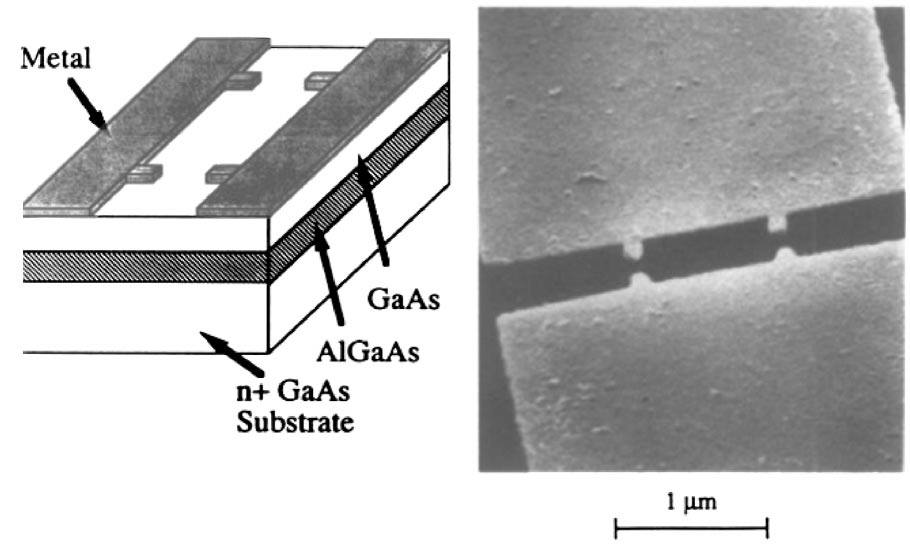
\includegraphics[width=\textwidth]{Figure_5_Reimann}
				\caption{Lateral quantum dot.}
		    \end{subfigure}
			\begin{subfigure}[t]{0.4\textwidth}
				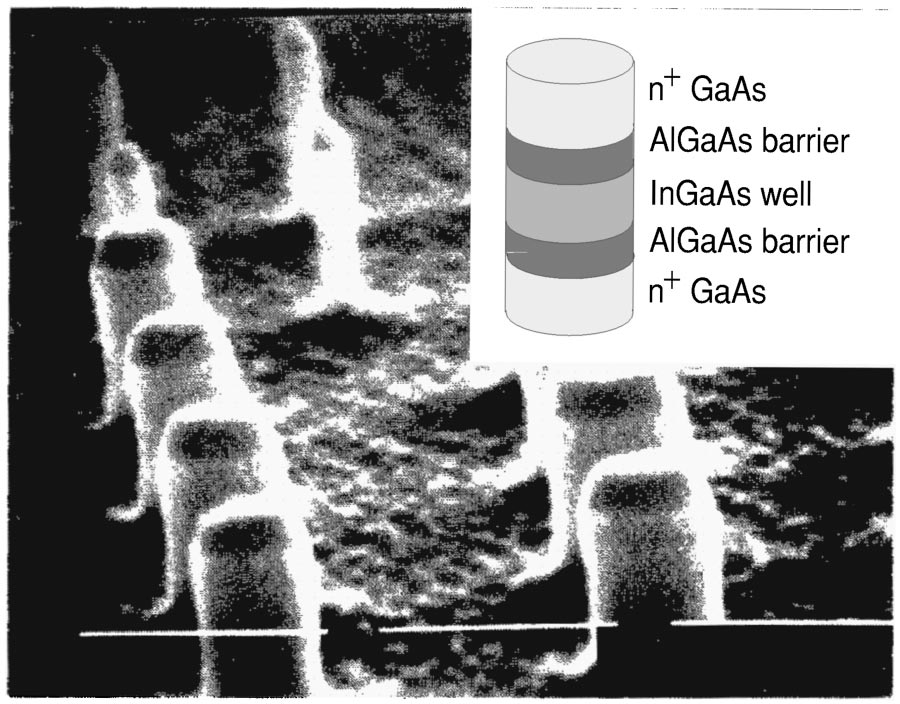
\includegraphics[width=\textwidth]{Figure_4_Reimann}
				\caption{Etched quantum dots.}
		    \end{subfigure}
		\end{figure}
	}
	
	\note{
		Quantum dots are built by stacking up different layers of semiconductors. The electron gas forms at the interface of different layers, and the confinement is obtained by applying a voltage to the top metal electrodes -- called \emph{gates}. In the Figure, the white bars have a length of $\SI{0.5}{\micro\meter}$.; so, the gates are created by lithographic patterning.

		Another common method to fabricate quantum dots is to build heterostructure pillars by etching techniques. Here, the electrodes are at the top and at the bottom of the pillars.

		Other fabricating processes include self-growth mechanisms, in which the growth conditions determine the form of the structure (that can be pyramidal, disk shaped or lens shaped), and cleaved-edge overgrowth, that consists in two separate Molecular Beam Epitaxy growths on a specific substrate.
	}
	
\end{frame}

\begin{versionLONG}

\begin{frame}{The single-electron transistor}

	\uncover<+->{A quantum dot can be schematized as a \emph{single-electron transistor}.}
	
	\uncover<+->{Its charge is a multiple of the elementary charge and transport proceeds one electron at the time.}
	
	\uncover<+->{
		\begin{figure}
			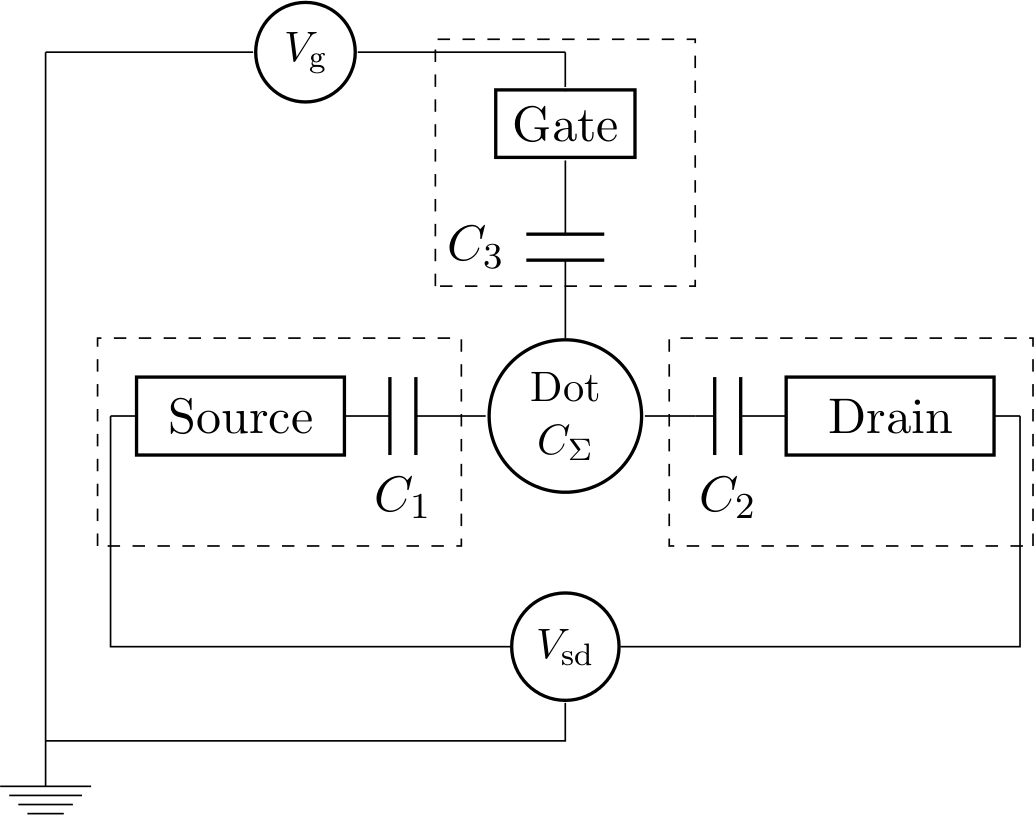
\includegraphics[width=0.6\textwidth]{SET}
		\end{figure}	
	}
	
	\note{
		\alert{READ THE SLIDE}.
		
		In figure, we have the scheme of a single electron transistor. The island has index 0, the source has index 1, the drain index 2 and the gate index 3. The capacitances are meant to be intrinsic capacitances of the respective electrode (source, drain or gate).
	}	
	
\end{frame}

\begin{frame}{The Coulomb blockade effect}

	\begin{itemize}[<+->]
		\item The electron island is weakly coupled with source and drain via tunnel barriers.
		\item When the thermal energy is not enough to make an electron tunnel the barriers, the conduction is blocked.
		\item This effect is called the \alert{Coulomb blockade}, and shows up in \emph{conductance} measurements.
	\end{itemize}
	
	\uncover<+->{
		\begin{figure}
			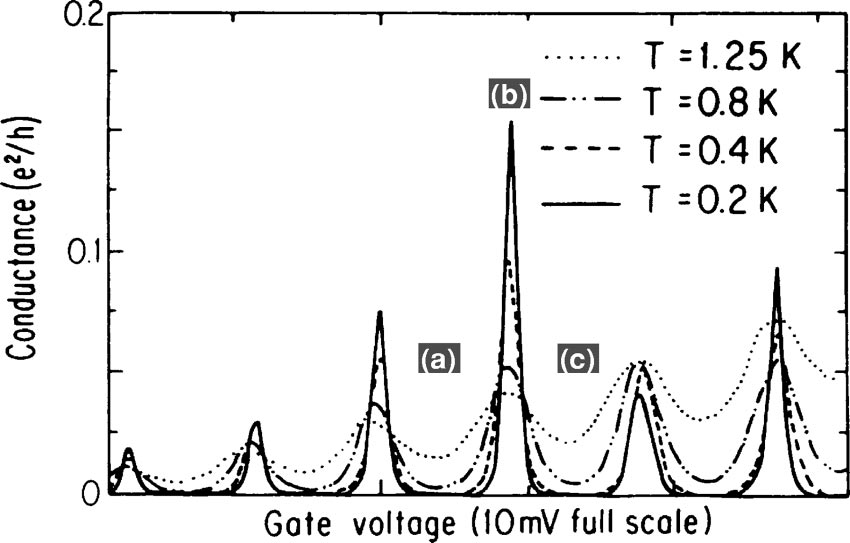
\includegraphics[width=0.6\textwidth]{Figure_6_Reimann}
		\end{figure}	
	}
	
	\note{		
		The behavior of a quantum dot can be analyzed by studying its electron transport mechanism. In order to do that, the dot is connected to a circuit that provides a certain gate voltage, and its conductance is measured.
		
		\alert{READ THE SLIDE}.
		
		A plot like the one in Figure (Coulomb oscillations in a lateral quantum dot) is obtained; you see that there are conductance peaks at specific gate voltages, all of them evenly spaced. This behavior can be explained by the \emph{Coulomb blockade model}.
	}
	
\end{frame}

\begin{frame}{The Coulomb blockade effect}
	
	\begin{figure}
		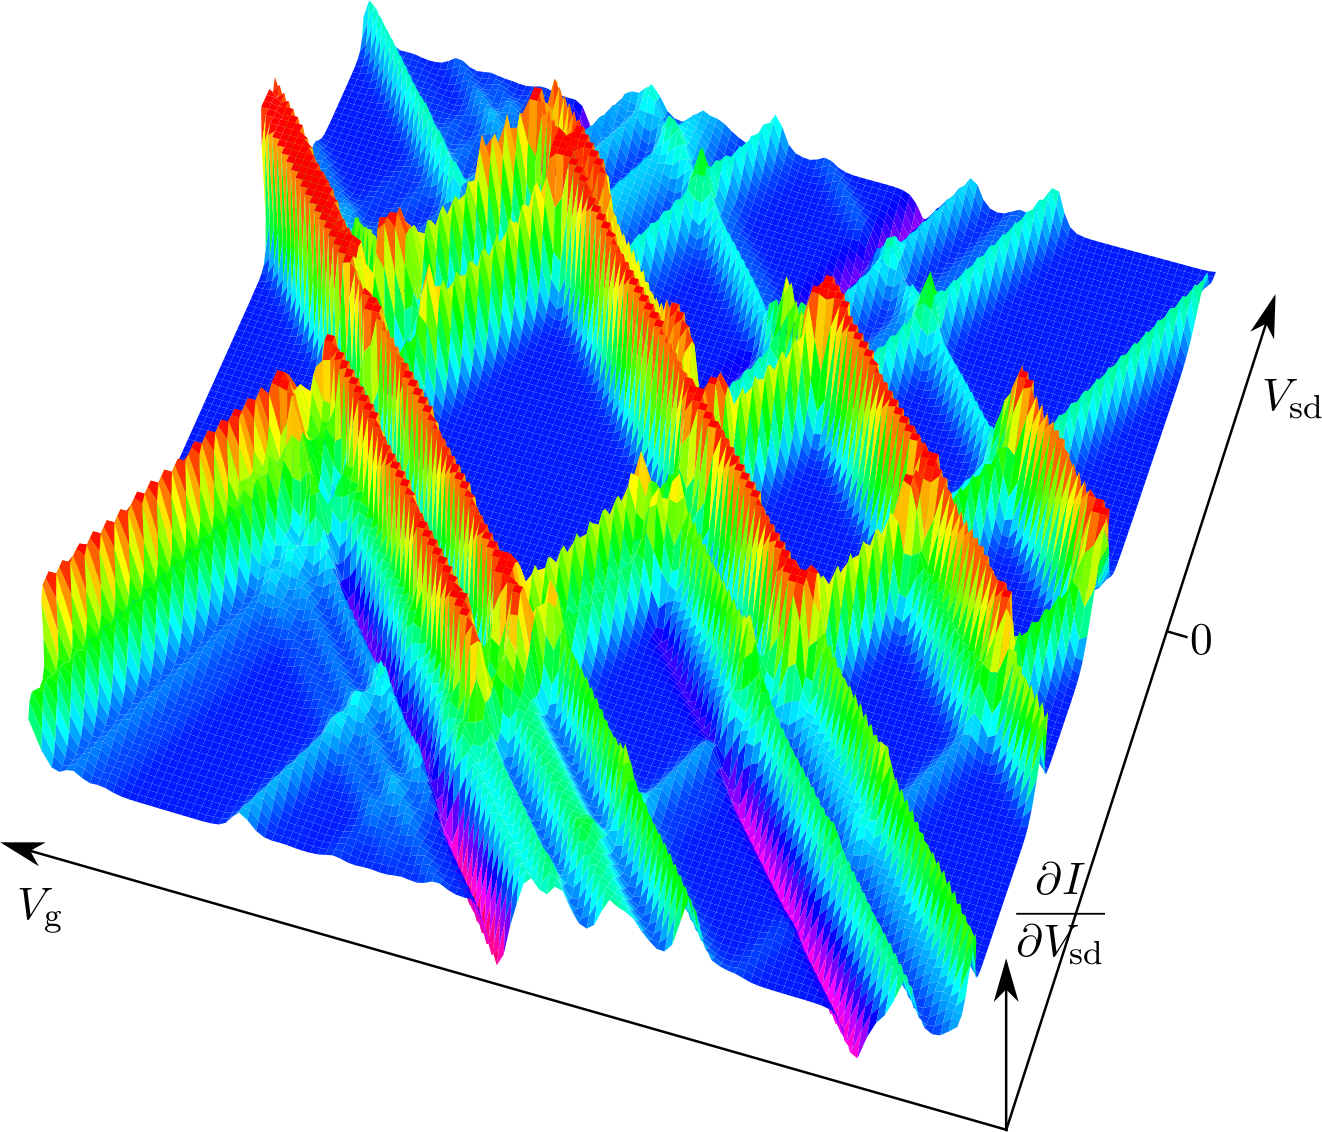
\includegraphics[width=0.6\textwidth]{diff_cond}
		\caption{Differential conductance measurements in a nanowire.}
	\end{figure}	
	
\end{frame}

\begin{frame}{Band diagram}

	\begin{figure}
		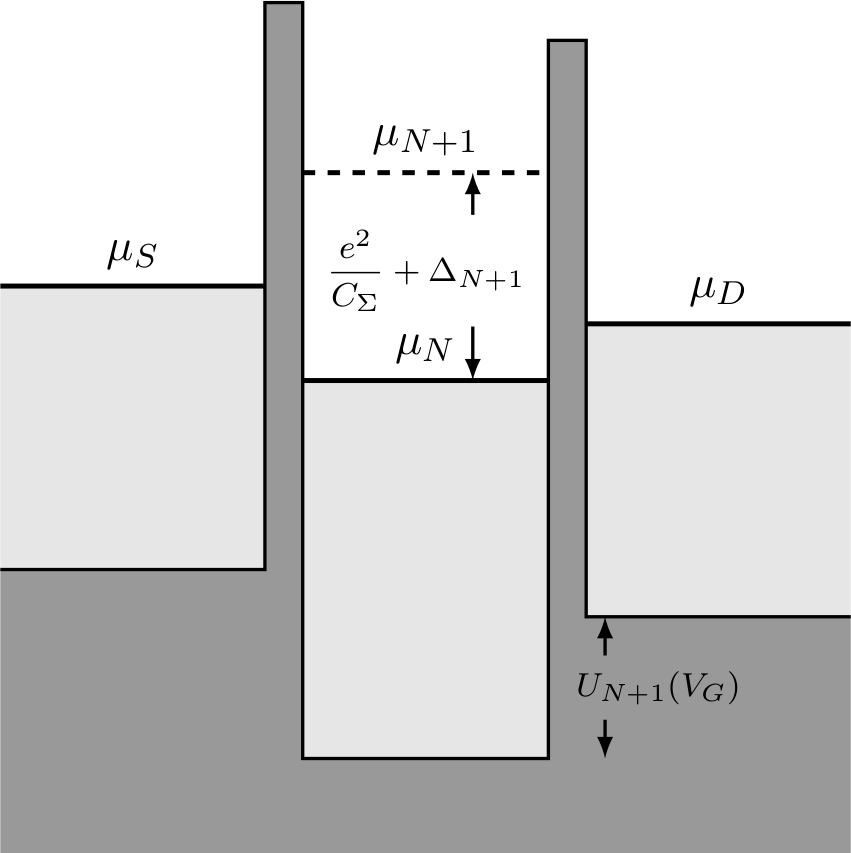
\includegraphics[width=0.6\textwidth]{SET_a}
	\end{figure}	
	
	\note{
		Let's see what happens in terms of the electrochemical potential.
		
		Let's consider the low-temperature, low-bias voltage case ($eV_{\text{bias}},k_BT \ll e^2/C_{\Sigma}$). Let's also suppose that, initially, the electrochemical potential inside the dot -- $\mu_N$ -- is lower than the electrochemical potential of the drain -- $\mu_D$: the transport is blocked due to the Coulomb blockade effect.
		
		The number of electrons inside the dot is $N$.
	}	
	
\end{frame}

\begin{frame}{Band diagram}

	\begin{figure}
		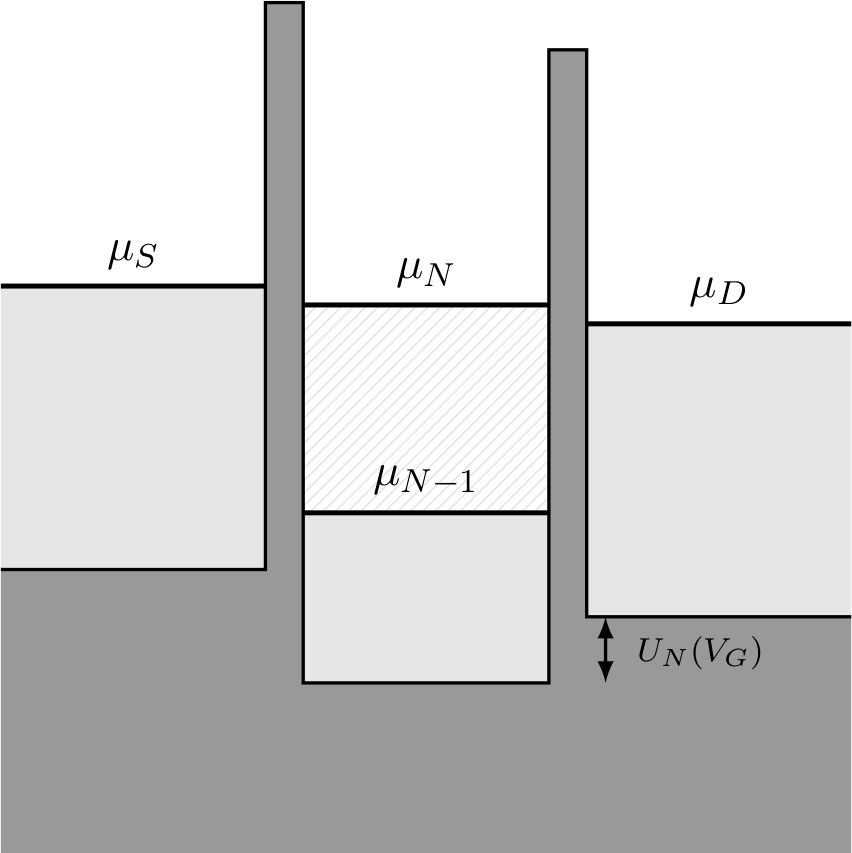
\includegraphics[width=0.6\textwidth]{SET_b}
	\end{figure}	
	
	\note{
		Now, we can decrease the gate voltage: the overall effect is that we have a linear increase in $\mu_N$ wrt the gate voltage. Eventually, $\mu_N$ will align to $\mu_D$ ($\mu_N = \mu_D$), which means that an electron can leave the dot. At the same time, if $\mu_S \gtrsim \mu_D$, an electron from $\mu_S$ can enter the dot; the overall effect is that the number of the electrons inside the dot oscillates between $N$ and $N-1$, and an electric current flows through the dot from the drain to the source. In terms of the conductance, this corresponds in a peak.
	}
	
\end{frame}

\begin{frame}{Band diagram}

	\begin{figure}
		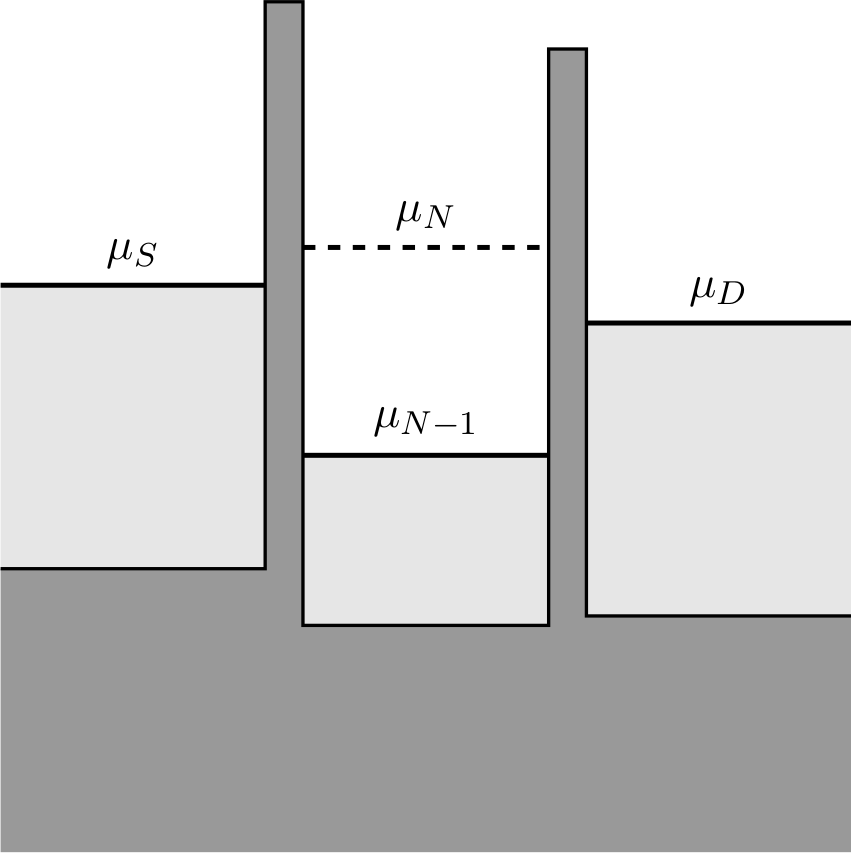
\includegraphics[width=0.6\textwidth]{SET_c}
	\end{figure}	
	
	\note{
		If we keep lowering the gate voltage -- i.e., increasing $\mu_N$ -- until $\mu_N > \mu_S$, then the dot is left with only $N-1$ electrons. Now, the level to consider is $\mu_{N-1}$: you see that it's far below $\mu_D$, so the current is blocked again.
	}
	
\end{frame}

\end{versionLONG}

\section{The algorithm}

\begin{frame}{The variational principle}
	
	\uncover<+->{The \alert{variational principle} is a powerful tool that allows, for \emph{any} system, to calculate an \emph{upper bound} estimate for the \emph{ground state} energy.}
	
	\uncover<+->{Being $E_{\text{gs}}$ the ground-state energy, $\Ket{\psi}$ a state whatsoever and $\hat{H}$ the Hamiltonian of the system, the principle states that}
	
	\uncover<+->{
		\begin{equation}
			E_{\text{gs}} \leq \frac{\Braket{\psi|\hat{H}|\psi}}{\Braket{\psi|\psi}}.
		\end{equation}
	}
	
	\uncover<+->{We are going to use this principle by calculating the quantity on the right hand side, for a chosen \emph{trial wave-function} $\psi_T$. We will come back later on how to guess a realistic $\psi_T$.}
	
	\note{
		The Variational Principle is a method of general validity that can be used to gather information about a system with a Hamiltonian that we are unable to diagonalize. Specifically, this principle gives us an \emph{upper bound} for the energy of the ground state. The formulation is really simple: if you pick \emph{any state $\Ket{\psi}$ whatsoever}, then \alert{SHOW FORMULA ON SLIDE}.
		
		In practice, one chooses a class of states for $\Ket{\psi}$ parametrized by one or more parameters -- the so-called \emph{variational parameters}, and then calculates the quantity $E_T$ for multiple sets of values of the variational parameters $\alpha_1\ldots,\alpha_n$. The lower value of $E_T$ obtained in this way is the required upper bound. If one manages to find an even lower value for $E_T$ with a more clever wave-function, then he has found a better upper bound for the ground state energy.

		The only trouble with this method is that we never know for sure how close we are to the \emph{actual} ground state energy; all we get for sure is just an upper bound. However, if one manages to guess a \emph{realistic} $\Ket{\psi}$, he often gets values for the ground state energy that miraculously match the actual ones.
	}
	
\end{frame}

\begin{frame}{The local energy}
	
	\uncover<+->{In the function-representation of the states, we can recast the above relation as}
	
	\uncover<+->{
		\begin{equation}
			E_{\text{gs}}
			\leq \int d\vec{\tau}\,\mathcal{P}(\vec{\tau})E_L(\vec{\tau})
			\simeq \frac{1}{n}\sum_{i=1}^{n}E_L(\vec{\tau}),
		\end{equation}
	}
	
	\uncover<+->{where}
	
	\uncover<+->{
		\begin{equation}
			\mathcal{P}(\vec{\tau}) = \frac{|\psi_T|^2}{\int d\vec{\tau} \, |\psi_T|^2}
			\qquad
			\text{and}
			\qquad
			E_L(\vec{\tau}) = \frac{1}{\psi_T} \hat{H} \psi_T.
		\end{equation}
	}
	
	\uncover<+->{The quantity $E_L$ is called the \alert{local energy}.}
	
	\note{
		Calculating $E_T$ as it appears in the previous relation is not a piece of cake. However, we can recast that equation in a simpler form as \alert{READ THE SLIDE}.
	}

\end{frame}

\begin{frame}{The local energy}
	
	\uncover<+->{Let's do a brief recap.}
	
	\begin{itemize}[<+->]
		\item Our upper bound is given by $\int d\vec{\tau}\,\mathcal{P}(\vec{\tau})E_L(\vec{\tau})$
		\item We can calculate it as $\frac{1}{n}\sum_{i=1}^{n}E_L(\vec{\tau})$ for a big enough $n$
		\item In other words, the idea is to sample tons of $E_L$ values at different positions in space and then take the mean
		\item Since the $E_L$'s have a certain distribution, we should sample more points where the probability is higher and less points where the probability is lower, in order to be sure to have a consistent set of samples.
		\item \alert{But how can we achieve such a distribution of samples?}
	\end{itemize}
	
\end{frame}

\begin{frame}{The Metropolis algorithm}

	\uncover<+->{The solution is to use the \alert{Metropolis algorithm}.}
	
	\uncover<+->{Let's suppose that we have just sampled $E_L$ at a certain point in space, let's call it $\vec{r}^{\text{old}}$.} \uncover<+->{Then, we make a \alert{random move} to another point in space, $\vec{r}^{\text{new}}$.}
	
	\uncover<+->{To check whether we moved to a higher probability region, we calculate the ratio of the respective probabilities, that is }
	
	\uncover<+->{
		\begin{equation}
			R 
			\doteqdot \frac{\mathcal{P}(\vec{r}^{\text{new}})}{\mathcal{P}(\vec{r}^{\text{old}})}
			= \frac{|\psi(\vec{r}^{\text{new}})|^2}{|\psi(\vec{r}^{\text{old}})|^2}.
		\end{equation}
	}
	
\end{frame}

\begin{frame}{The Metropolis algorithm}
	
	\uncover<+->{Then}
	
	\begin{itemize}[<+->]
		\item If $R \geq 1$, we accept this move because we are moving to a higher probability region and we sample $E_L$ in the new position.
		\item If $R < 1$, we can't blindly reject this move just because we are moving to a lower probability region; after all, we also have to populate the tails of the distribution! However, we can't accept all of this kind of moves.
	\end{itemize}
	
	\uncover<+->{\emph{Solution}: generate a random number $r \in (0,1)$, and accept the move (i.e., sample $E_L$) if $r \leq R$. Otherwise, the sample is rejected.}
	
	\uncover<+->{This procedure is known as the \alert{brute force} Metropolis algorithm.}

\end{frame}

\begin{frame}{The Metropolis algorithm}
	
	\uncover<+->{Let's recap it:}
	
	\begin{itemize}[<+->]
		\item Choose a starting position $\vec{r}^{\text{old}}$ and a step-length $l$.
		\item Generate a random number $\varepsilon$ in the interval $(0,1)$ and compute a new position $\vec{r}^{\text{new}} = \vec{r}^{\text{old}} + l\varepsilon$.
		\item Compute the acceptance ratio $R = \frac{|\psi_T(\vec{r}^{\text{new}})|^2}{|\psi_T(\vec{r}^{\text{old}})|^2}$.
		\item Generate a new random number $r$ in the interval $(0,1)$.
		\item If $R \geq r$, accept the step and store the position by letting $\vec{r}^{\text{old}} = \vec{r}^{\text{new}}$.
		\item If $R < r$, reject the step and  discard the position by letting $\vec{r}^{\text{new}} = \vec{r}^{\text{old}}$.
	\end{itemize}
	
\end{frame}

\begin{frame}{Choose the proper step-length}

	\uncover<+->{\alert{Problem:}} \uncover<+->{we have \emph{no rule} to say what a proper step length should be.}
	
	\begin{itemize}[<+->]
		\item If it's \emph{too much}, our walker will make huge jumps all around and will sample very few points inside our distribution; the measurement will not be good.
		\item If it's \emph{too less}, our walker will wander around the starting point and will not cover all the distribution space; the measurement will not be good as well.
	\end{itemize}
	
	\uncover<+->{\alert{Solution:}} \uncover<+->{as a \emph{rule of thumb}, one can test different step lengths and then choose the one that gives an acceptance of around $\SI{50}{\percent}$.}
	
	\note{
		So far, we haven't specified any rule for the choice of the step length. \alert{READ LIST}.
	}

\end{frame}

\begin{frame}{Importance sampling}

	\uncover<+->{A clever approach is to implement the \alert{importance sampling.}}
	
	\uncover<+->{\emph{Idea:} use the knowledge about the system to improve the acceptance ratio $R$.}
	
	\note{An improved acceptance ratio wastes less points.}
	
	\uncover<+->{Procedure:}
	\begin{itemize}[<+->]
		\item Recast the Schr\"{o}dinger equation a \emph{diffusion problem}, in which the walker is pushed in those regions where the trial wave-function is larger.
		\item The force $\vec{F}$ responsible for pushing the walker is called the \emph{quantum force}, and can be expressed as
		\uncover<+->{
			\begin{equation}
				\vec{F}=2\frac{1}{\psi_T}\nabla\psi_T
			\end{equation}
		}
	\end{itemize}
	
	\note{
		A better approach is to implement the \emph{Importance sampling}, that consists in doing more clever assumptions on the shape of the transition probability.
		
		Since we know the system we are working on, we know that if we recast the Schr\"{o}dinger equation as a diffusion problem, the transition probability is going to be a Gaussian distribution (or a modified Gaussian).
		
		The driving force of this diffusion problem is called the \emph{quantum force}, and can be expressed as \alert{SHOW THE FORMULA}.
	}

\end{frame}

\begin{frame}{Importance sampling}

	\begin{itemize}[<+->]
		\item The new position is calculated as
		\uncover<+->{
			\begin{equation}
				r^{\text{new}} = r^{\text{old}} + D\vec{F}(r^{\text{old}})\Delta t + \varepsilon,
			\end{equation}
		}
		\uncover<+->{where $\Delta t$ is a chosen time-step and $D=0.5$ is the diffusion constant.}
		\item The improved acceptance ratio can be expressed as
		\uncover<+->{
			\begin{equation}
				R = \frac{|\psi_T(r^{\text{new}})|^2G(r^{\text{old}},r^{\text{new}},\Delta t)}{|\psi_T(r^{\text{old}})|^2G(r^{\text{new}},r^{\text{old}},\Delta t)}.
			\end{equation}
		}
		\uncover<+->{where $G(x,y,\Delta t)$ is the Green's function}
		\uncover<+->{
			\begin{equation}
				G(y,x, \Delta t) = \dfrac{1}{(4 \pi D \Delta t)^{3N/2}} \exp(-(y - x - D \Delta t F(x))^2 / 4 D \Delta t).
			\end{equation}
		}
	\end{itemize}
	
	\note{
		
		\alert{READ THE NEW POSITION.}
		
		Here, the random variable $\varepsilon$ is no more uniform! For importance sampling, it's a \emph{Gaussian} random variable.
		
		\alert{CONTINUE READING.}
	}

\end{frame}

\section{The 2-electrons system}

\begin{frame}{The unperturbed system}

	\uncover<+->{Hamiltonian of the system:}
	
	\uncover<+->{
		\begin{equation}
			\hat{H}_0 = 
			\sum_{i=1}^{2} \left( -\frac{1}{2}\nabla_i^2 + \frac{1}{2}\omega^2r_i^2 \right),
		\end{equation}
	}
	
	\uncover<+->{Energy of a single electron in a 2D harmonic potential:}
	
	\uncover<+->{
		\begin{equation}
			E_{s} = \hbar\omega(n_x+n_y+1).
		\end{equation}
	}
	
	\note{
		Let's apply this algorithm to two electrons in an harmonic oscillator, without the electron-electron repulsion.
		
		The unperturbed Hamiltonian is \alert{SHOW THE HAMILTONIAN}.
		
		Unlike the one-dimensional case, for two dimensions we need two quantum numbers: $n_x$ and $n_y$ for the $x$ and $y$ directions, respectively, and this causes a degeneracy in the energy levels. The principal quantum number is $n=n_x+n_y$.
		
		For a single electron in a 2D harmonic potential, the energy can be expressed as \alert{SHOW THE ENERGY}.
	}

\end{frame}

\begin{frame}{The unperturbed system}
	
	\uncover<+->{Configuration:}
	
	\uncover<+->{
		\begin{figure}
		\centering
		\definecolor{myblue}{rgb}{0,0.447,0.741}	
		\begin{tikzpicture}
			\tikzset{>=latex}
			\draw [ultra thick] (-1,0) -- (1,0) node[midway,below,align=center] {\scriptsize $n_x=0$ \\ \scriptsize $n_y=0$};
			\draw [very thick, myblue, ->] (-0.5,-0.5) -- (-0.5,0.5);
			\draw [very thick, myblue, ->] (0.5,0.5) -- (0.5,-0.5);
		\end{tikzpicture}
		\end{figure}
	}
	
	\uncover<+->{Ground-state energy of the system, in natural units:}
	
	\uncover<+->{
		\begin{equation}
			E_{\text{gs}}=2\omega.
		\end{equation}
	}
	
	\uncover<+->{Exact wave-function:}
	
	\uncover<+->{
		\begin{equation}
			\phi(\vec{r}_1,\vec{r}_2) = C \exp\left(-\omega\left(r_1^2 + r_2^2\right)/2\right).
		\end{equation}
	}

	\note{
		This is the configuration of the system.
		
		You see that the spatial parts of the wave-functions are equal because of the spin degeneracy, so the ground state energy of the complete system has a factor of 2 to take this thing into account.
		
		For the same reason, the exact wave-function (or at least, its spatial part) can be expressed as the product of the single-particle wave-functions.
		
		$C$ is a normalization constant.
	}
	
\end{frame}

\begin{frame}{The unperturbed system}
	
	\uncover<+->{Since we know the exact wave-function, the problem is trivial. We choose our trial wave-function as}
	
	\uncover<+->{
		\begin{equation}
			\psi_T(\vec{r}_1,\vec{r}_2) = \exp\left(-\alpha\omega\left(r_1^2 + r_2^2\right)/2\right).
		\end{equation}
	}
	
	\uncover<+->{where $\alpha$ is a \alert{variational parameter}.}
	
	\uncover<+->{For $\alpha=1$ we expect to obtain a variational energy \alert{exactly} equal to the ground state energy $E_{\text{gs}}=2\omega$.}
	
	\note{
		Since we know the exact wave-function, the problem is trivial. 
		
		We model our trial wave-function by adding a variational parameter $\alpha$.
		
		For $\alpha=1$ we expect to obtain a variational energy \alert{exactly} equal to the ground state energy $E_{\text{gs}}=2\omega$.
		
		In other words, for $\alpha=1$ the upper bound given by the variational principle coincides with the \emph{true} ground state energy.
	}
	
\end{frame}

\begin{frame}{$\omega=1$}
	
	\begin{figure}
		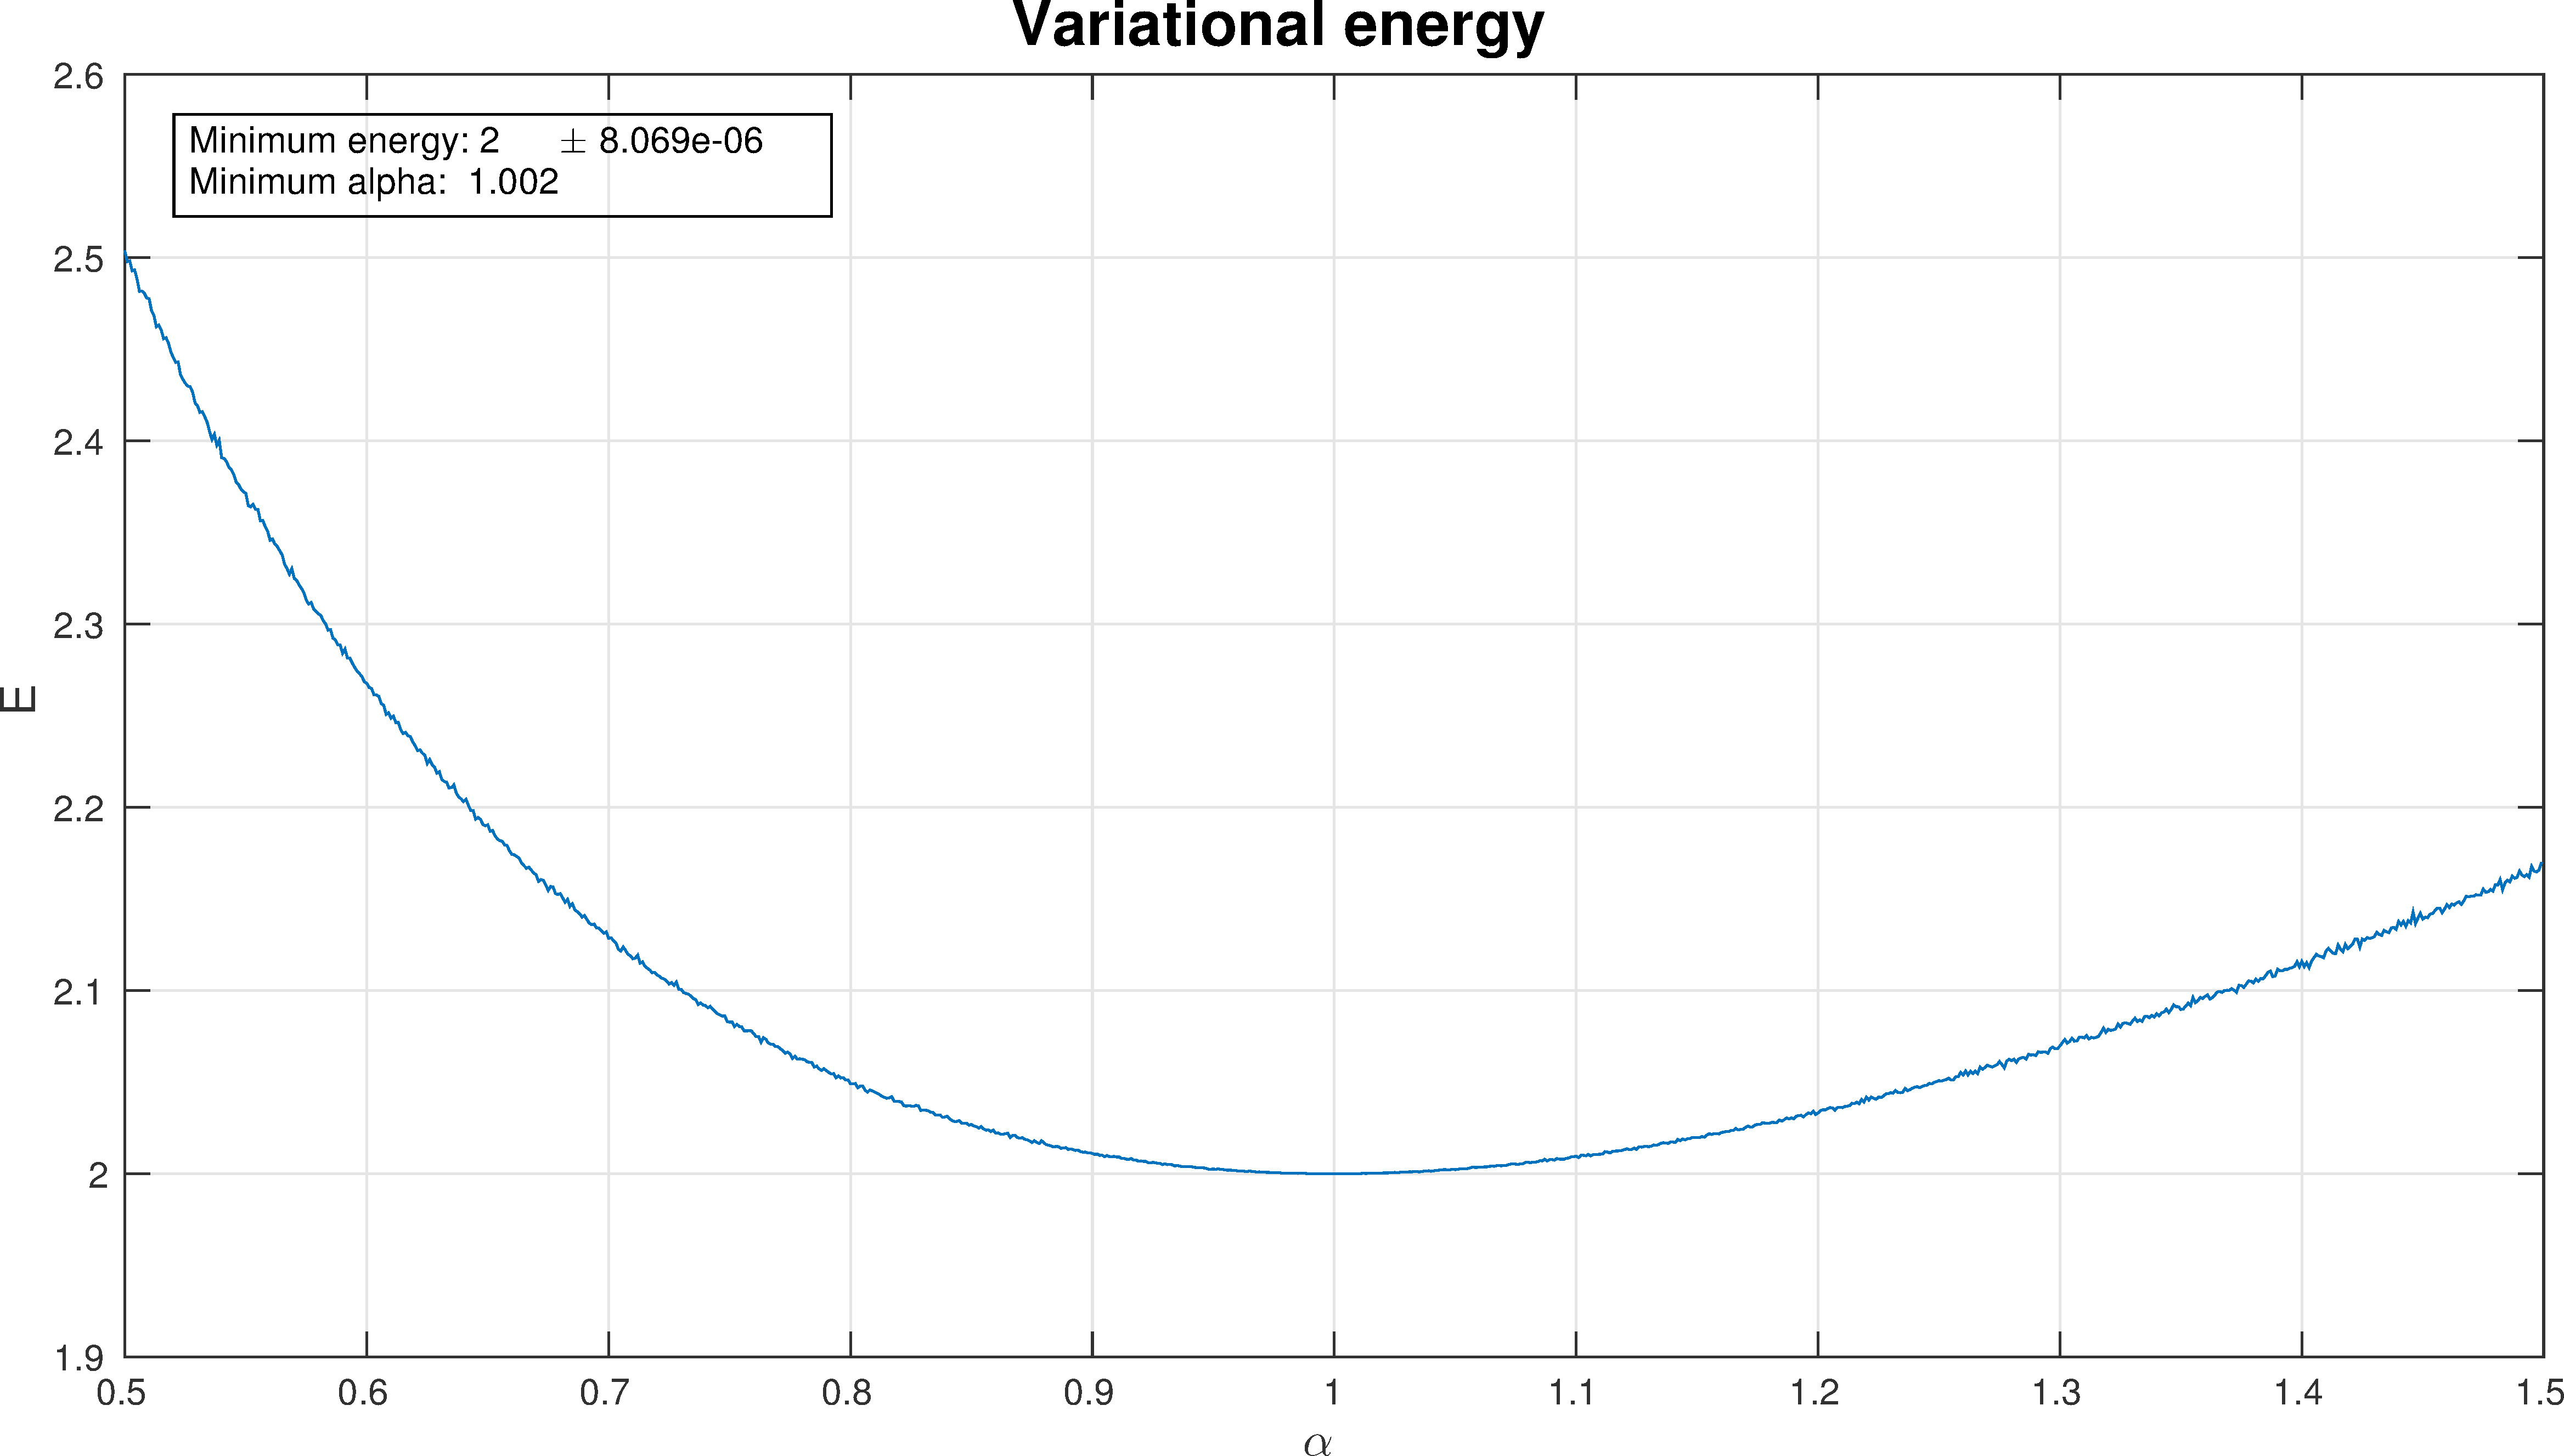
\includegraphics[width=\textwidth]{2e-norep}
	\end{figure}
	
	\note{
		The variational energy versus the variational parameter $\alpha$. The settings used are: brute force sampling with step length 2, no Jastrow factor, no parallelization, $1000$ variations of $\alpha$ around $1$ with step $0.001$, $\SI{1e7}{}$ Monte Carlo steps. Acceptance ratio varies from $40$ to $\SI{60}{\percent}$.
	}	
	
\end{frame}

\begin{frame}{The complete system}

	\uncover<+->{The full Hamiltonian is}
	
	\uncover<+->{
		\begin{equation}
			\hat{H}=-\frac{1}{2} \nabla^2_1 - \frac{1}{2} \nabla^2_2+\frac{1}{2}\omega r_1^2+\frac{1}{2}\omega r_2^2+ \frac{1}{|\vec{r_1}-\vec{r_2}|}.
		\end{equation}			
	}
	
	\uncover<+->{\alert{Problem:}} \uncover<+->{the term
	\begin{equation}
		\frac{1}{|\vec{r_1}-\vec{r_2}|}
	\end{equation}
	could be a division by zero.
	}
	
	\uncover<+->{\emph{Solution:}} \uncover<+->{add, in the wave-function, a factor that cancels the divergence in the Hamiltonian.}	
	
	\note{
		The Hamiltonian of the full system, that includes the electron-electron repulsion, has an extra term that diverges when the two particles are near to each other.
		
		The divergence can be canceled if we are smart in the choice of the wave-function, by adding a term that compensates the singularity.
	}
	
\end{frame}

\begin{frame}{The complete system}
	
	\uncover<+->{The extra factor is usually modeled as}
	
	\uncover<+->{
		\begin{equation}
			\exp\left( \frac{ar}{1+\beta r} \right)
		\end{equation}
	}
	
	\uncover<+->{that is called the \alert{Padé-Jastrow} factor.}
	
	\uncover<+->{$r$ is the inter-particle distance, $a$ is a parameter that depends on the spin, while $\beta$ is a \emph{variational parameter}.}
	
	\uncover<+->{For $\omega=1$ we get the upper bound $E=3$, that is compatible with the \emph{actual} ground state energy.}
	
	\note{
		An extra factor to the non-interacting wave-function is added, that has the form \alert{READ THE SLIDE}.
		
		In two dimensions
		\begin{equation}
			a = 
			\begin{cases}
				1 & \text{anti-parallel spin} \\
				1/3 & \text{parallel spin}
			\end{cases}
		\end{equation}
		
		The calculated upper bound coincides with the ground state energy calculated by Taut theoretically.
	}	
	
\end{frame}

\begin{frame}{The complete system}
	
	\begin{figure}
		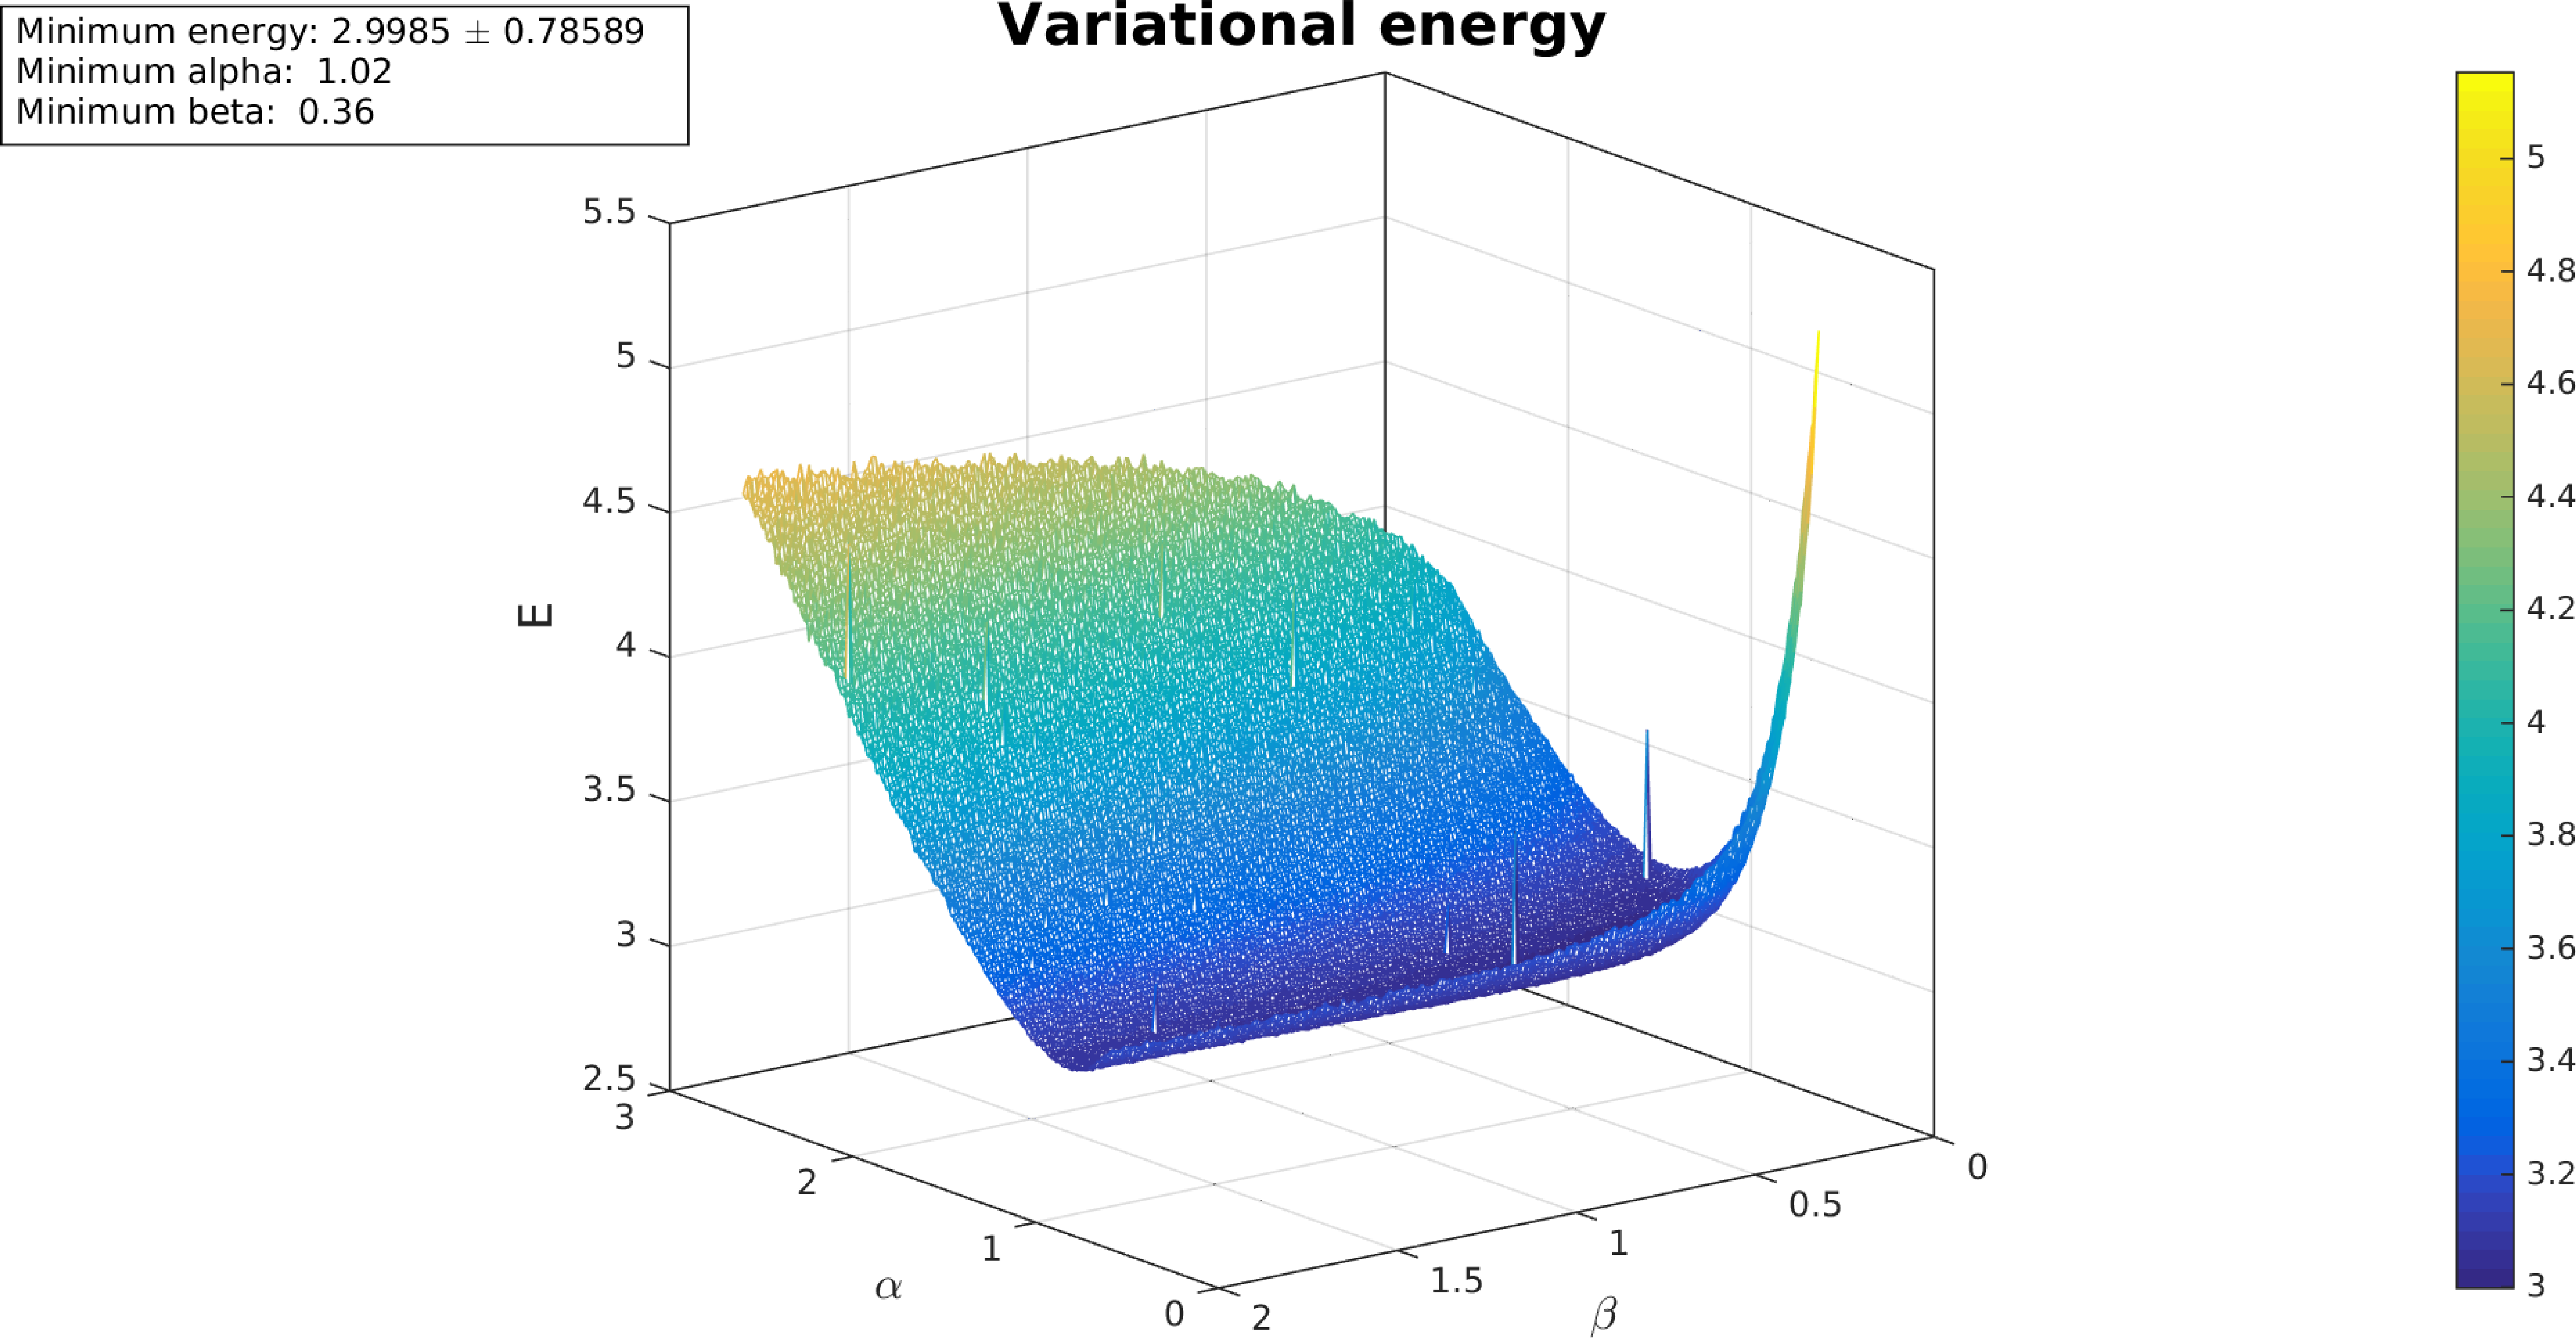
\includegraphics[width=\textwidth]{2e-rep}
	\end{figure}
	
	\note{
		The variational energy versus the variational parameters $\alpha$ and $\beta$. The settings used are: brute force sampling with step length 2, Jastrow factor, no parallelization, $200$ variations of $\alpha$ and $\beta$ with step $0.01$, $\SI{1e5}{}$ Monte Carlo steps. Acceptance ratio varies from $45$ to $\SI{55}{\percent}$.
	}

\end{frame}

\begin{frame}{The complete system}
	
	\begin{figure}
		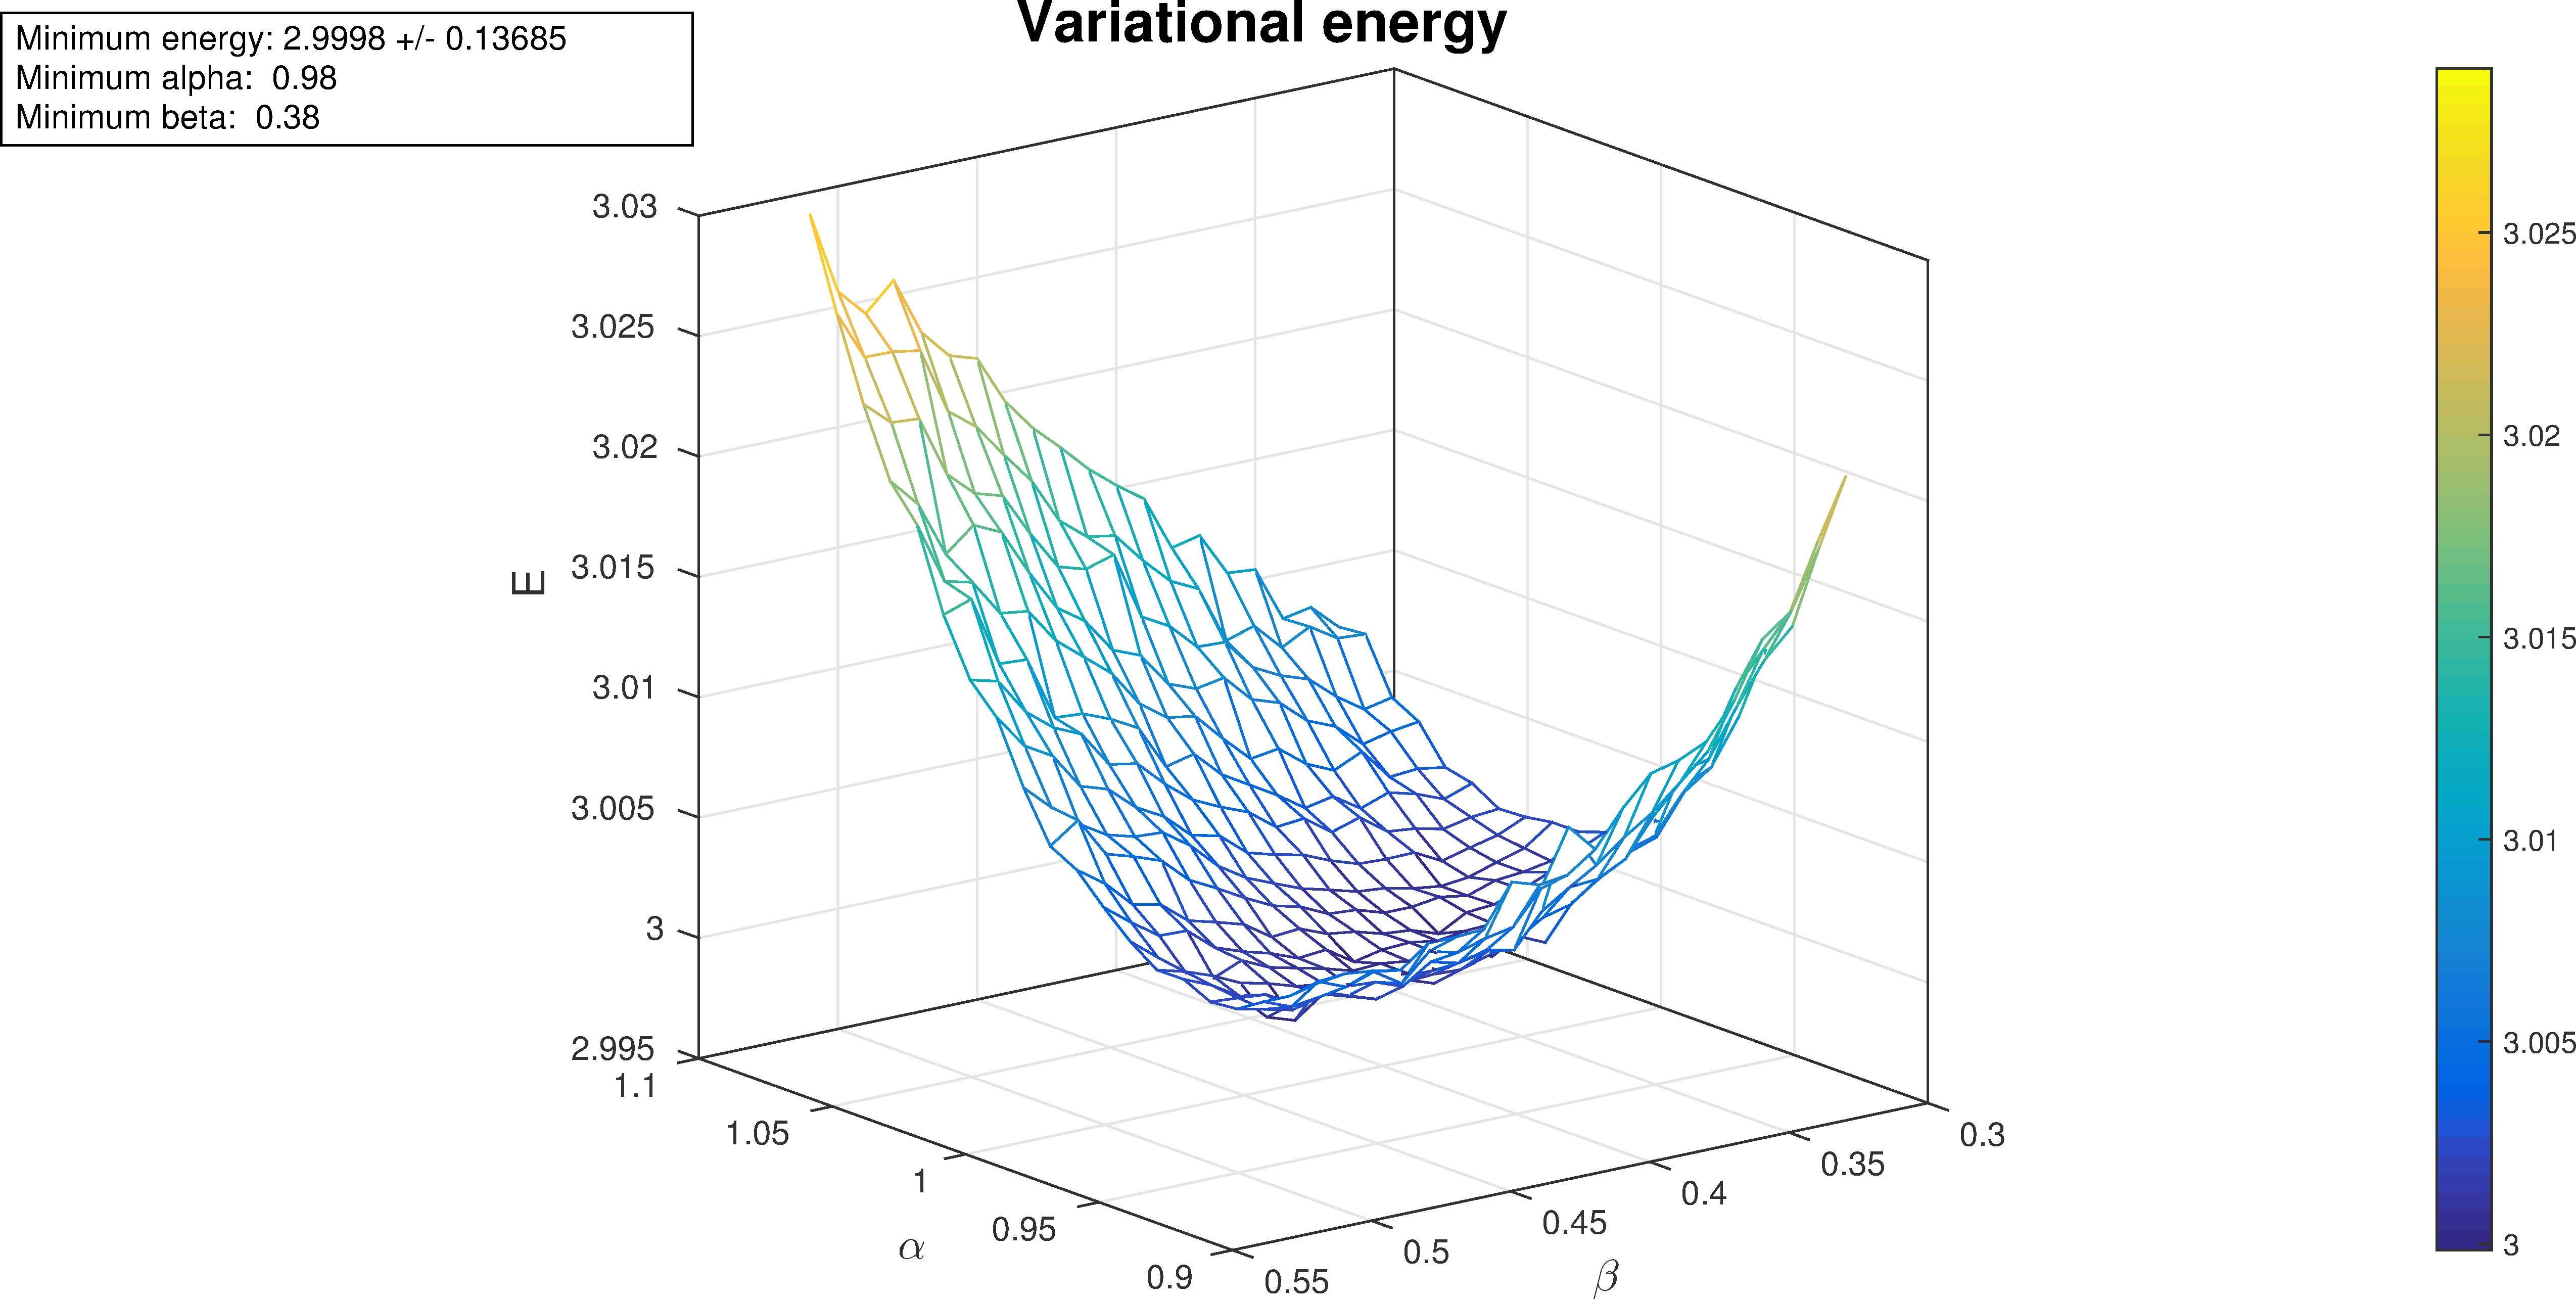
\includegraphics[width=\textwidth]{2e-rep_fine}
	\end{figure}
	
	\note{
		The variational energy versus the variational parameters $\alpha$ and $\beta$. The settings used are: brute force sampling with step length 2, Jastrow factor, no parallelization, $20$ variations of $\alpha$ and $\beta$ with step $0.01$, $\SI{1e6}{}$ Monte Carlo steps. Acceptance ratio varies from $45$ to $\SI{55}{\percent}$. The relative distance is about $\SI{1.64}{}$ in natural units.
	}

\end{frame}

\begin{frame}{Parallelization}

	\uncover<+->{\emph{Idea:} take multiple measurements for each point in order to lower the error.}
	
	\uncover<+->{If we take $n$ measurements of the same quantity, its error falls like}
	
	\uncover<+->{
		\begin{equation*}
			 \frac{1}{\sqrt{n}}
		\end{equation*}
	}
	
	\uncover<+->{We obtain more precise energy values even with less Monte Carlo steps.}
	
	\note{
		Despite the fact that we have very good values, you see that the error is still quite large.
		
		We can improve it by taking multiple measurements at each point of the grid, and then take the mean. If we do that, the error falls like the $1/\sqrt{n}$ and we can obtain more precise energy values even with less Monte Carlo steps.
	}

\end{frame}

\begin{frame}{$\omega=1$}

	\begin{figure}
		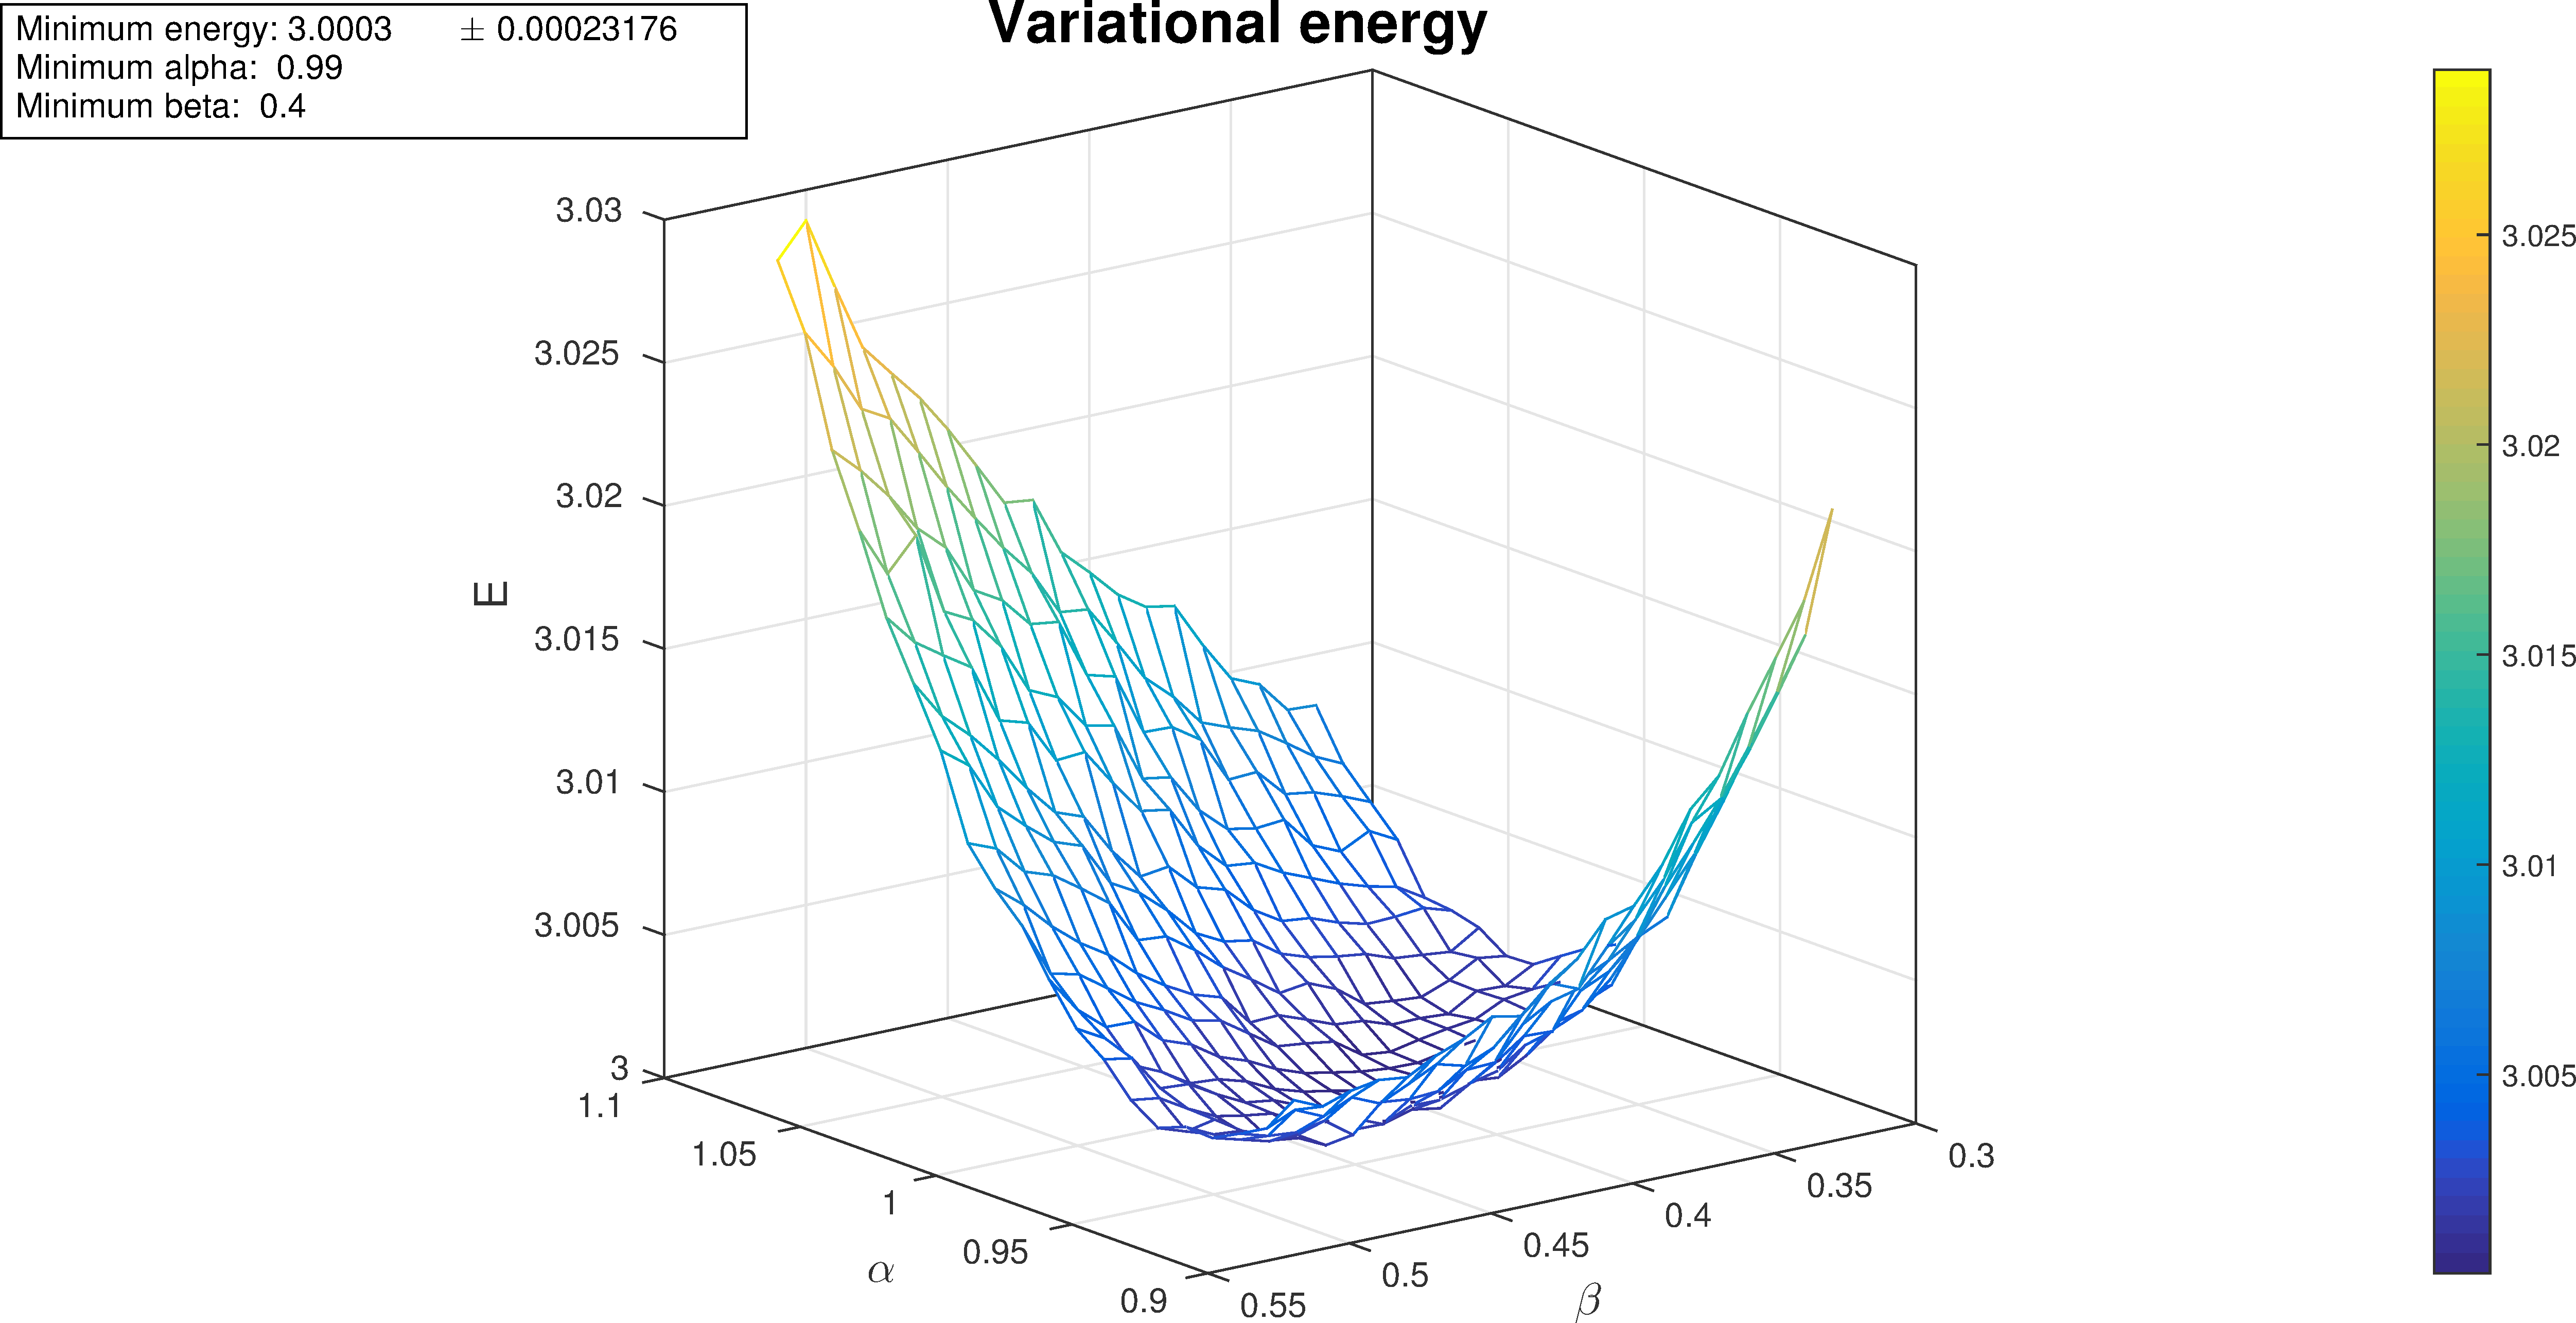
\includegraphics[width=\textwidth]{2e-rep_parallel}
	\end{figure}
	
	\note{
		The variational energy versus the variational parameters $\alpha$ and $\beta$. The settings used are: brute force sampling with step length 2, Jastrow factor, parallelization (8 threads), $20$ variations of $\alpha$ and $\beta$ with step $0.01$, $\SI{2e5}{}$ Monte Carlo steps. Acceptance ratio varies from $45$ to $\SI{55}{\percent}$.
	}

\end{frame}

\begin{frame}{Importance sampling}
	
	\uncover<+->{\emph{Idea:} implement importance sampling in order to waste less points.}
	
	\uncover<+->{\alert{Problem:}} \uncover<+->{if the time-step is too small and we don't use enough Monte Carlo steps, we have bad data.}
	
	\uncover<+->{\emph{Reason:} the walker remains near its starting point and will not cover completely the integration space.}
	
	\uncover<+->{\alert{Solution:}}
	\begin{itemize}[<+->]
		\item For a given time-step, increase the number of Monte Carlo cycles until the acceptance ratio is slightly below $\SI{100}{\percent}$.
		\item For a given number of Monte Carlo cycles, increase the time-step until the acceptance ratio is slightly below $\SI{100}{\percent}$.
	\end{itemize}
	
	\note{
		A further improvement would be to implement the importance sampling, as explained in the previous section.
		
		The only thing we have to care about is the amount of the time-step. \alert{READ THE SLIDE.}
		
		The solution is to test different values for the time-step and use the one that gives an acceptance ratio that is slightly below $\SI{100}{\percent}$.
	}
	
\end{frame}

\begin{frame}{$\omega=1$}

	\begin{figure}
		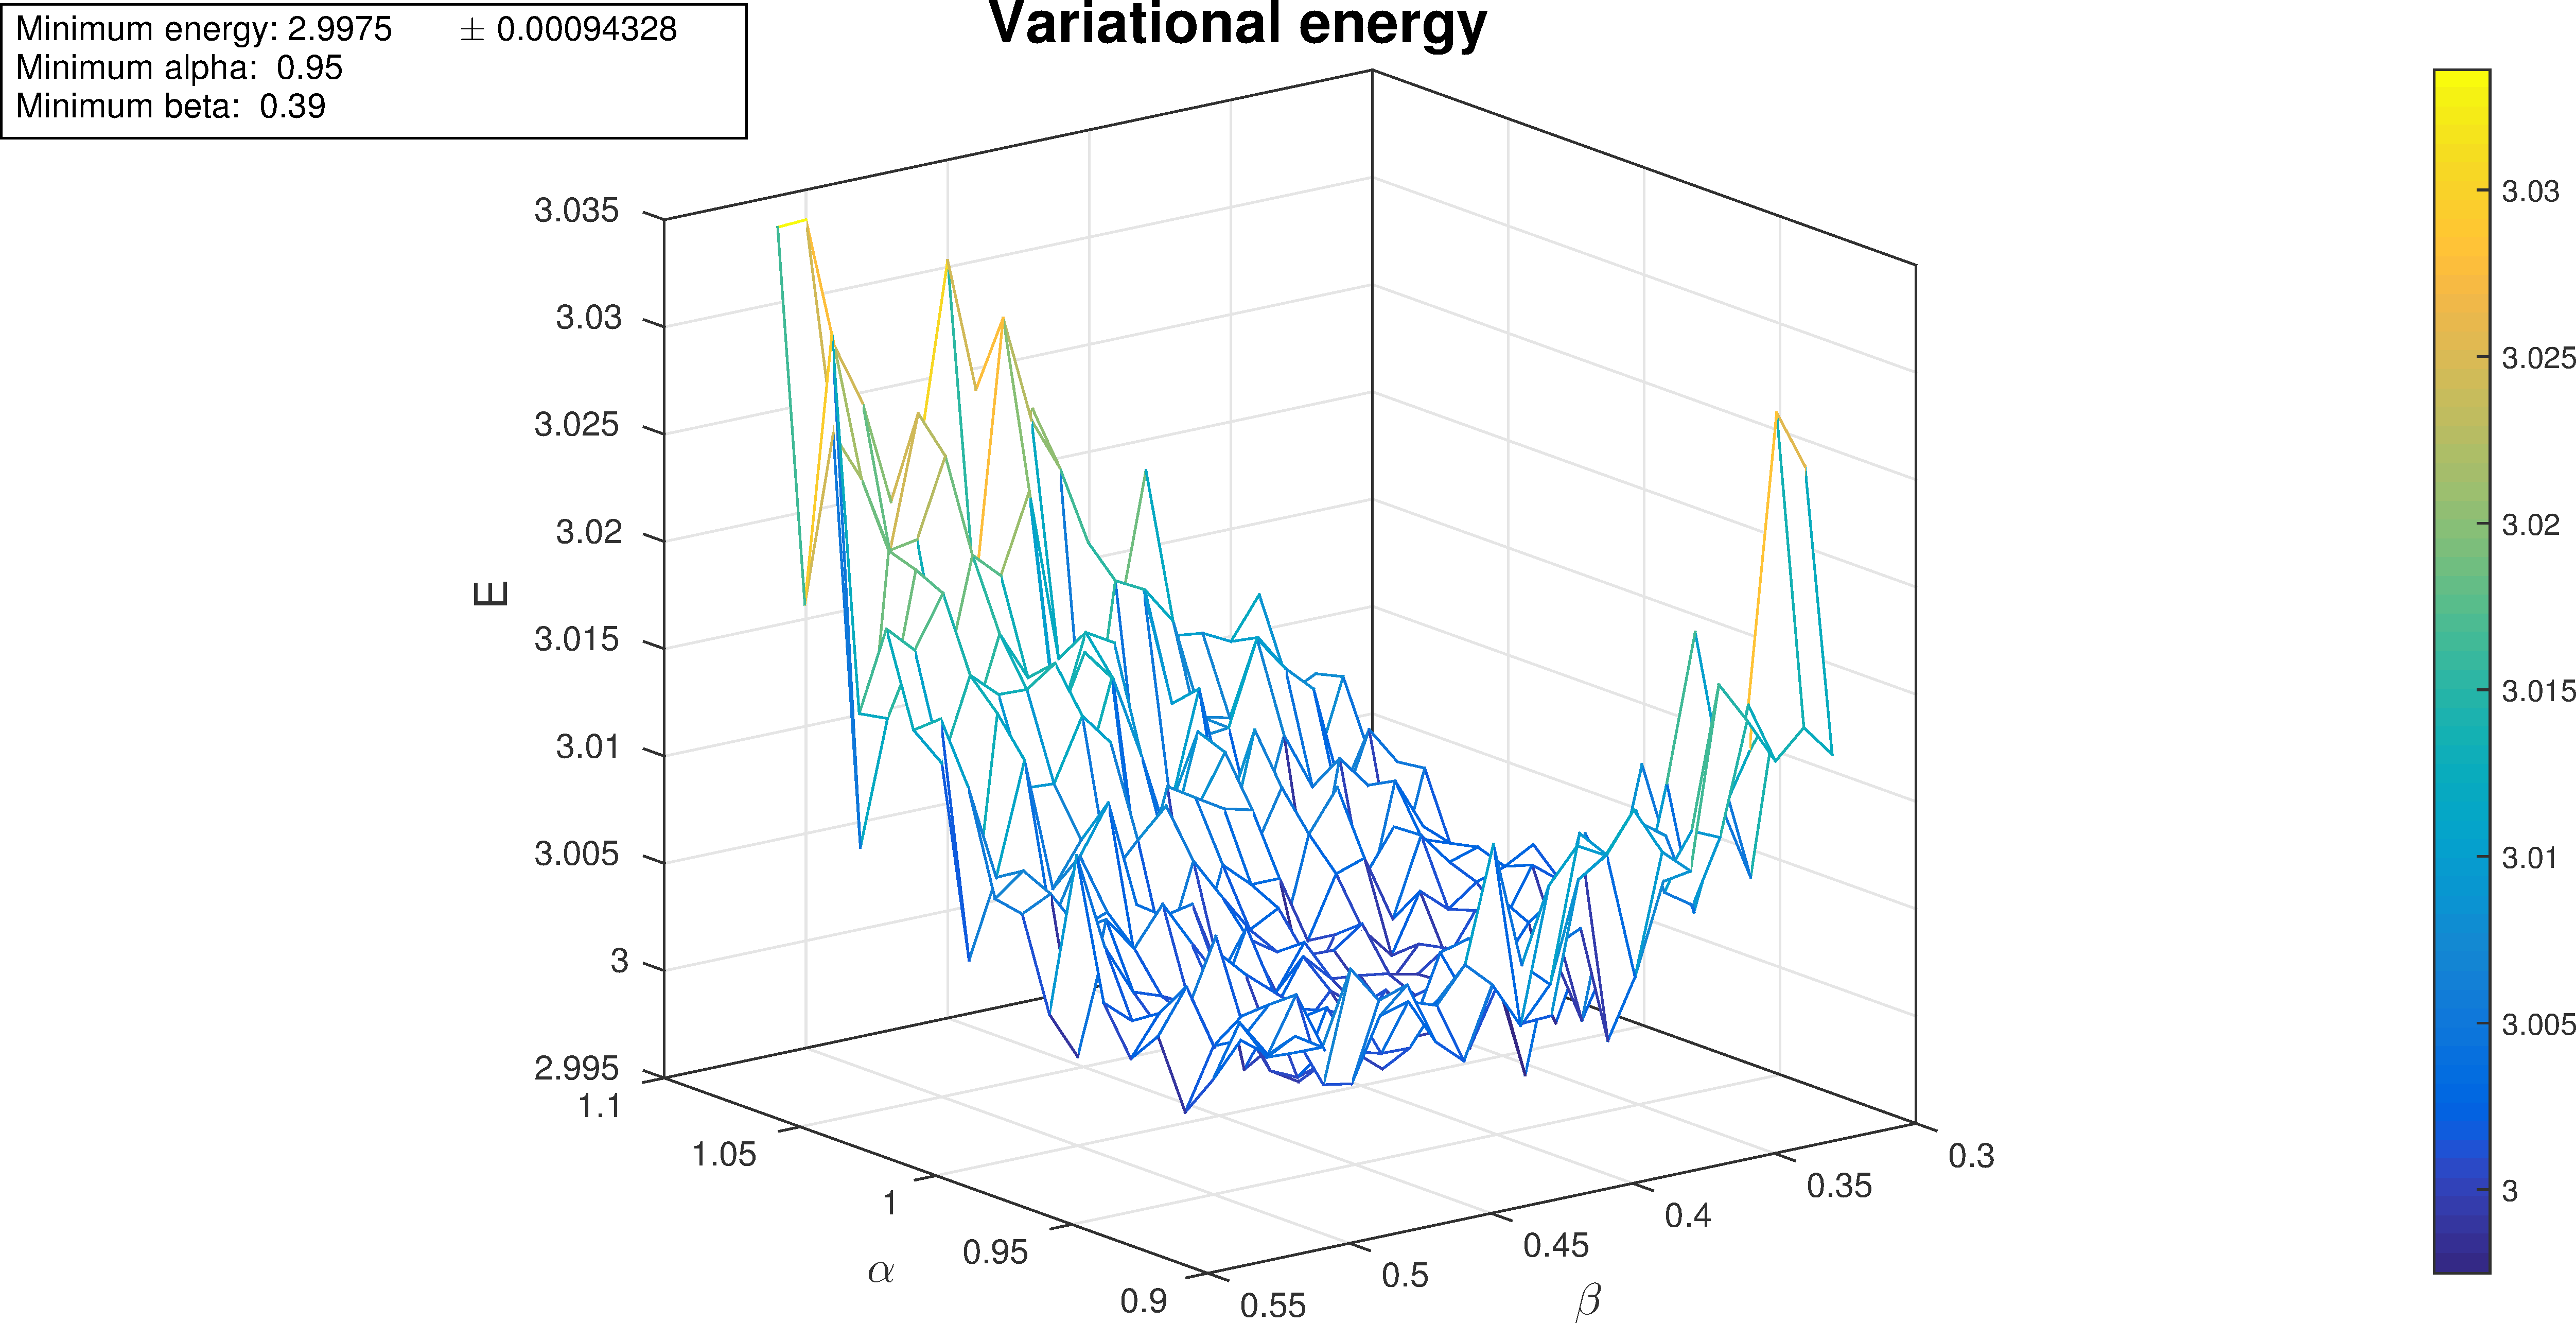
\includegraphics[width=\textwidth]{2e-rep_imp_small}
	\end{figure}
	
	\note{
		The variational energy versus the variational parameters $\alpha$ and $\beta$. The settings used are: importance sampling with $\Delta t = 0.001$, Jastrow factor, parallelization (8 threads), $20$ variations of $\alpha$ and $\beta$ with step $0.01$, $\SI{2e5}{}$ Monte Carlo steps. Acceptance ratio is about $\SI{99.999}{\percent}$.
		}
	
\end{frame}

\begin{frame}{$\omega=1$}

	\begin{figure}
		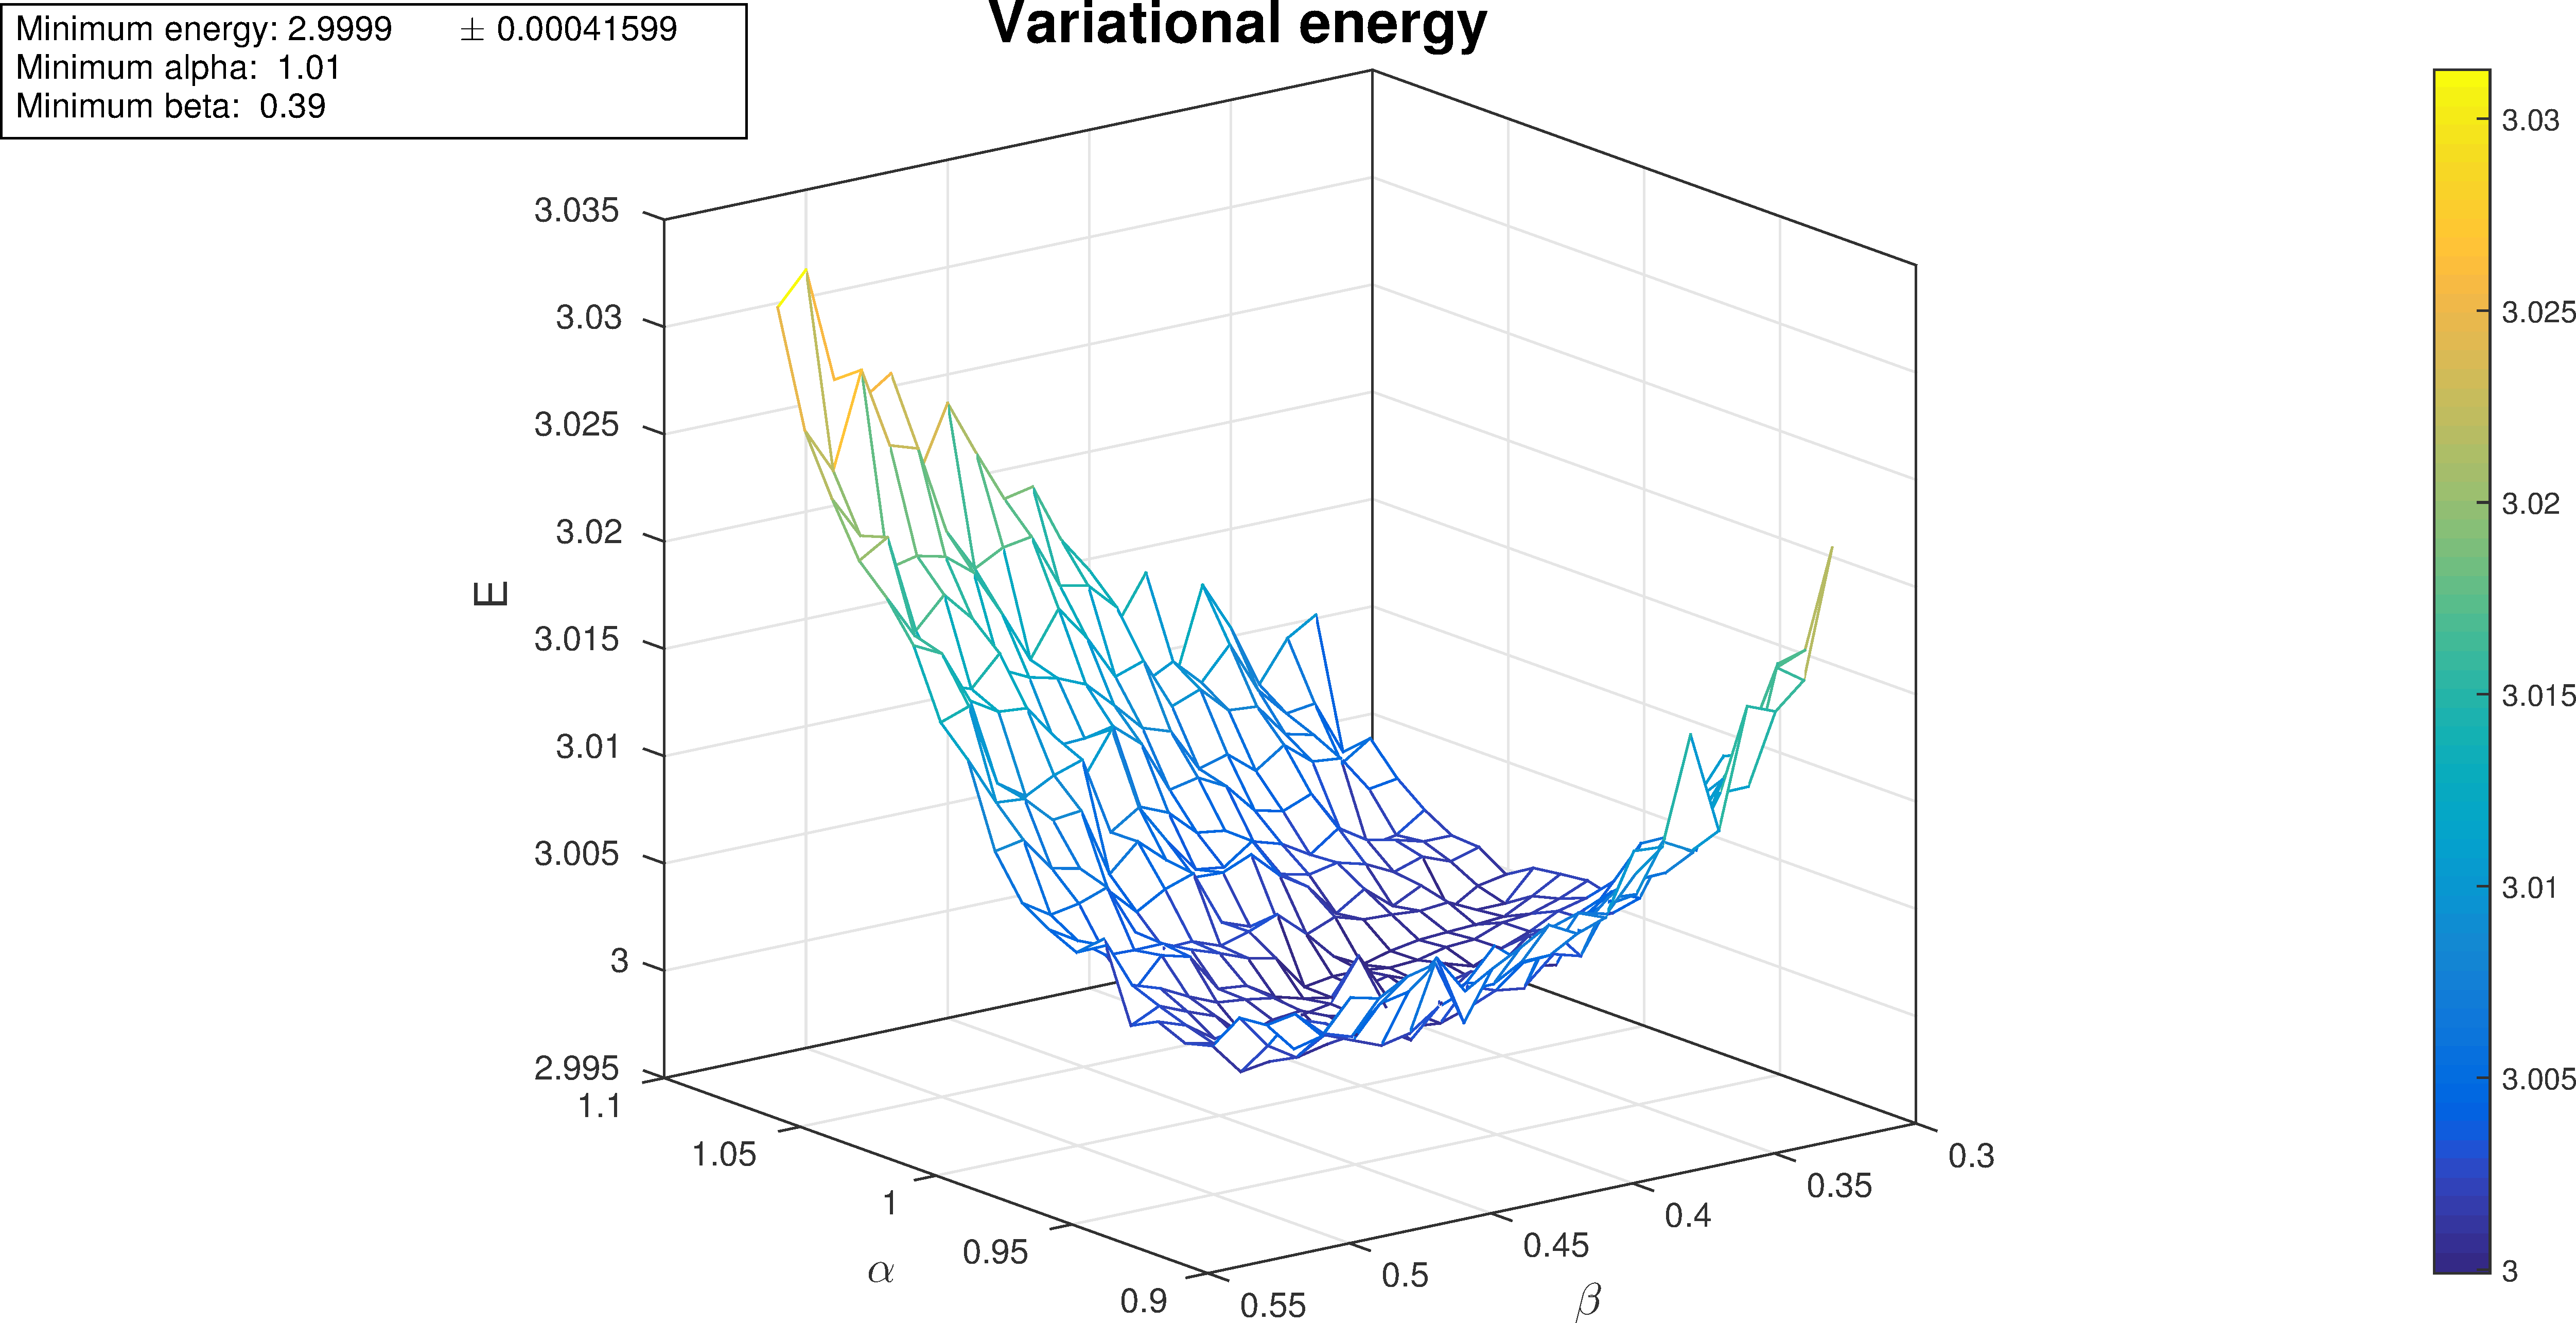
\includegraphics[width=\textwidth]{2e-rep_imp_med}
	\end{figure}
	
	\note{
		The variational energy versus the variational parameters $\alpha$ and $\beta$. The settings used are: importance sampling with $\Delta t = 0.01$, Jastrow factor, parallelization (8 threads), $20$ variations of $\alpha$ and $\beta$ with step $0.01$, $\SI{2e5}{}$ Monte Carlo steps. Acceptance ratio is about $\SI{99.999}{\percent}$.
		}
	
\end{frame}

\begin{frame}{$\omega=1$}

	\begin{figure}
		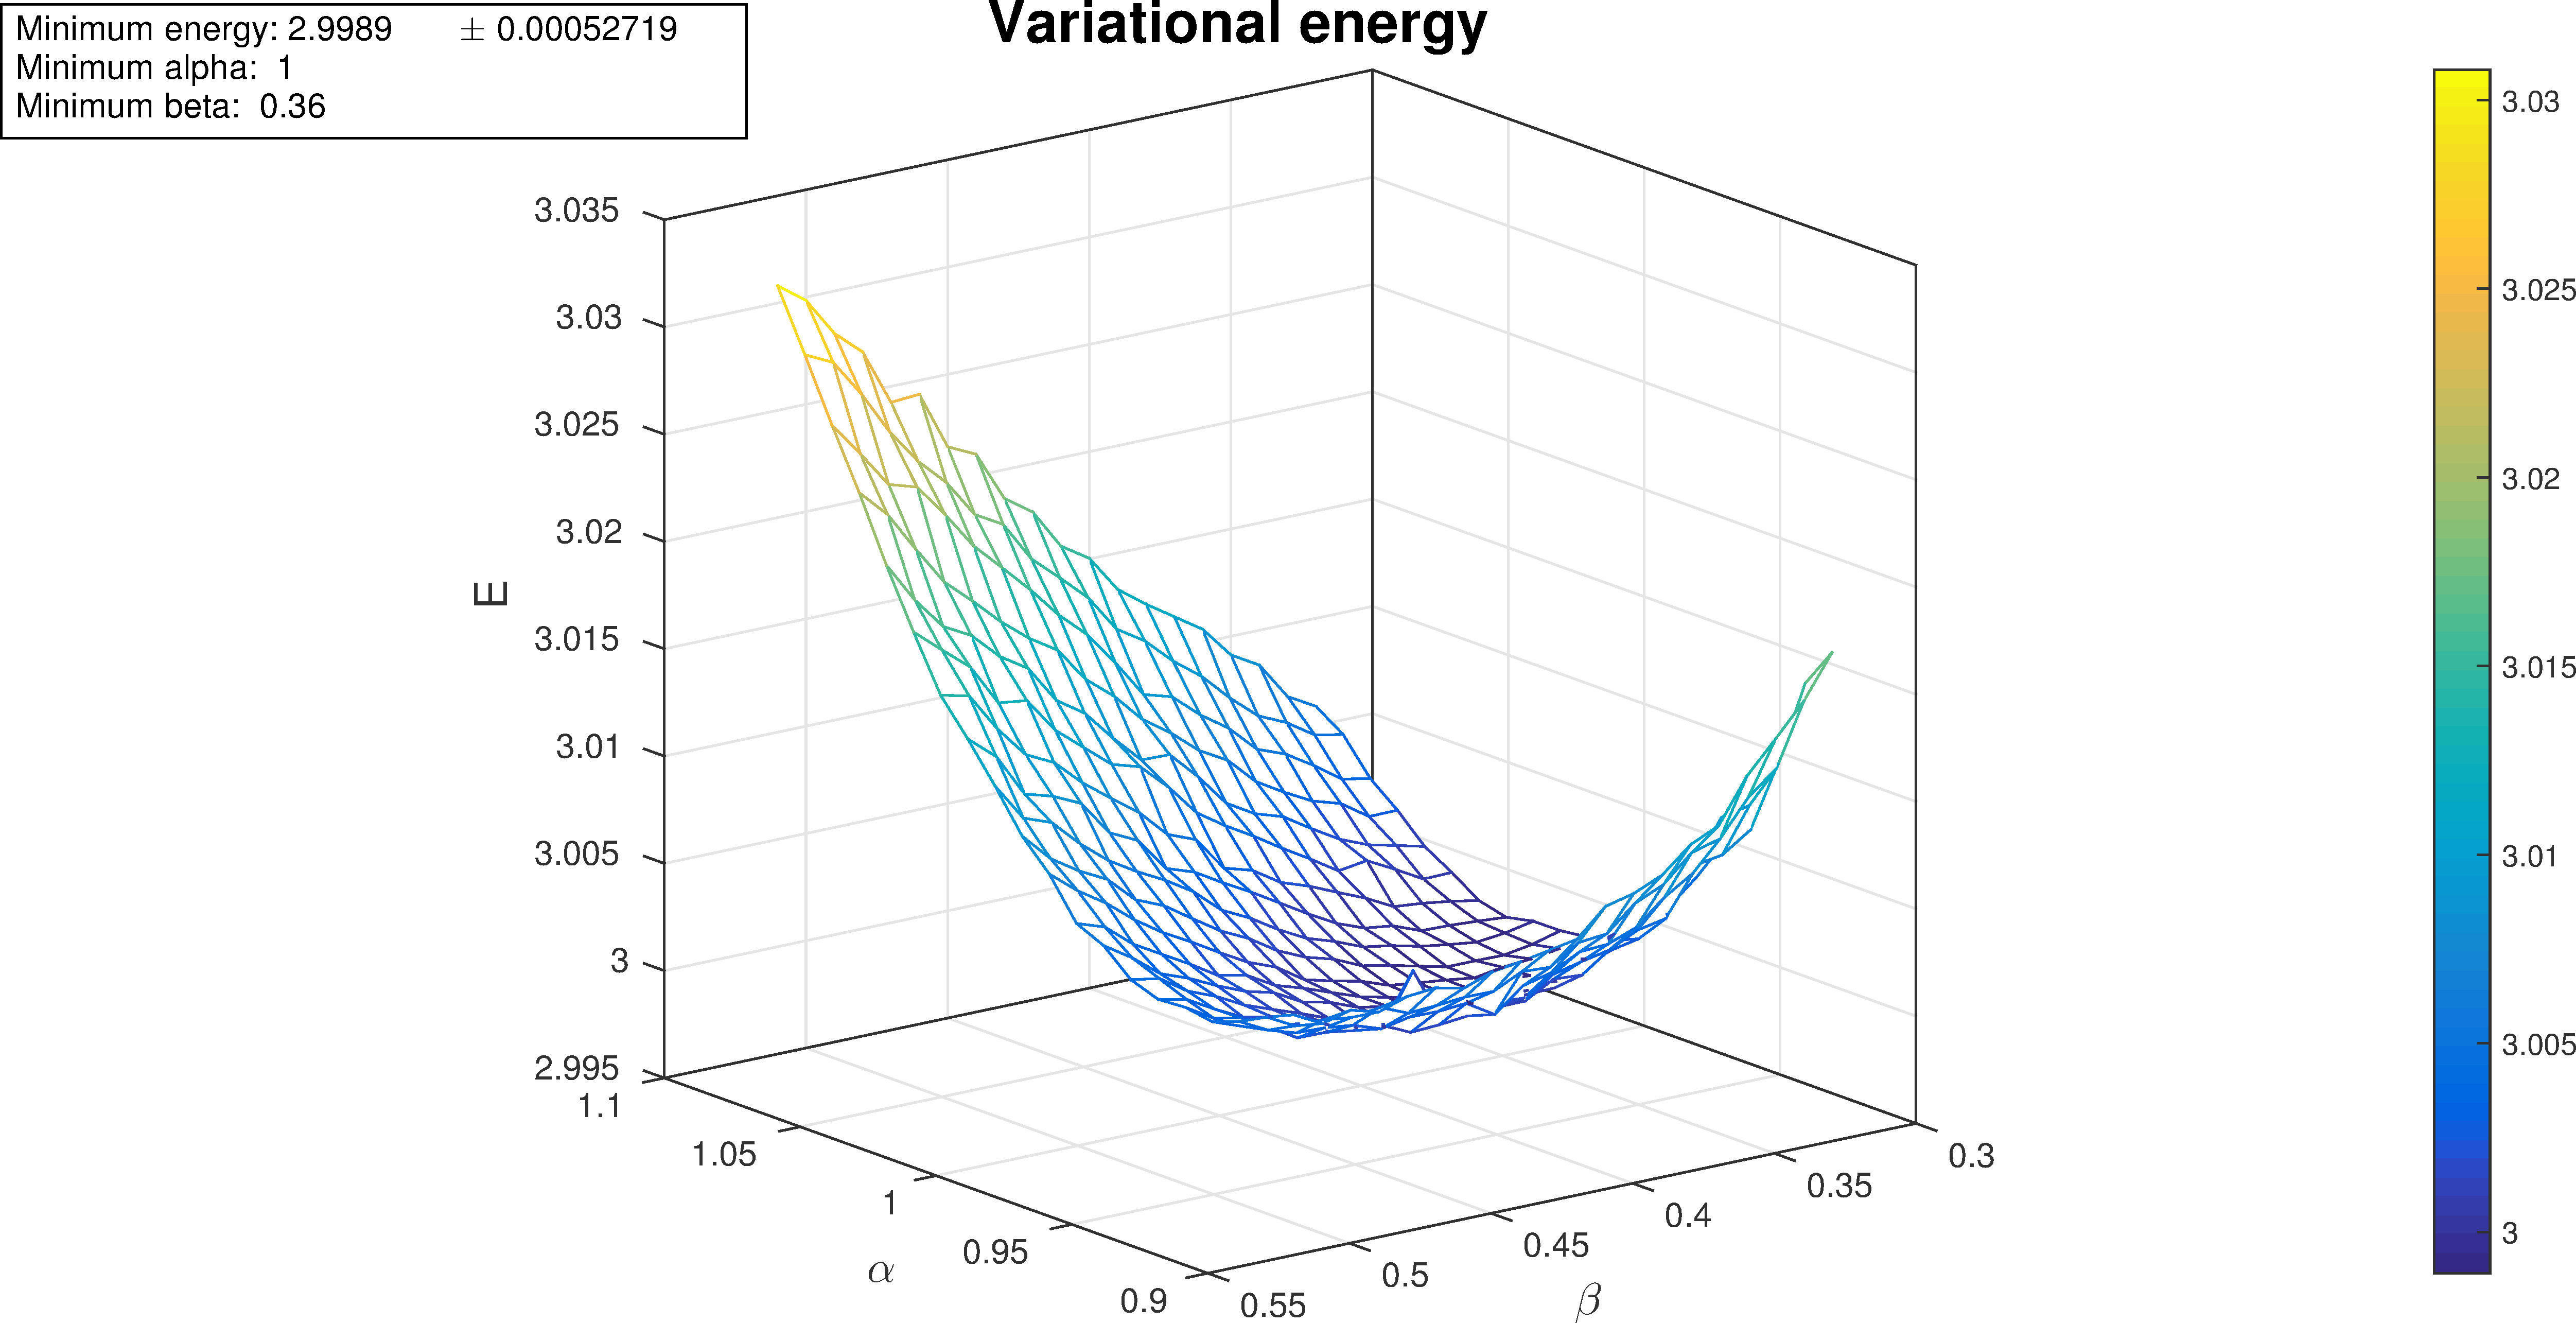
\includegraphics[width=\textwidth]{2e-rep_imp_high}
	\end{figure}
	
	\note{
		The variational energy versus the variational parameters $\alpha$ and $\beta$. The settings used are: importance sampling with $\Delta t = 0.1$, Jastrow factor, parallelization (8 threads), $20$ variations of $\alpha$ and $\beta$ with step $0.01$, $\SI{2e5}{}$ Monte Carlo steps. Acceptance ratio is about $\SI{99.793}{\percent}$.
		}
	
\end{frame}

\section{The 6-electrons system}

\begin{frame}{The trial wave-function}
	
	\uncover<+->{The trial wave-function is like the one we used for 2 electrons, but this time is more general.}
	
	\uncover<+->{For 2 electrons, it was}
	\uncover<+->{
		\begin{equation}
			\psi_T(\vec{r}_1,\vec{r}_2) 
			= \phi(\vec{r}_1)\phi(\vec{r}_2)\exp\left(\frac{ar_{12}}{1+\beta r_{12}}\right)
		\end{equation}
	}
	
	\uncover<+->{where $\phi$ is the single-particle spatial wave-function for $(n_x,n_y)=(0,0)$, that is equal for both electron $1$ and electron $2$, and $r_{12}$ is the inter-particle distance}.
	
\end{frame}

\begin{frame}{The trial wave-function}

	\uncover<+->{For $N$ electrons, the generalization is straightforward:}
	
	\uncover<+->{
		\begin{equation}
			\psi_T(\vec{r}_1,\ldots,\vec{r}_N) 
			= |S|\prod_{i<j}^{N}\exp\left(\frac{ar_{ij}}{1+\beta r_{ij}}\right)
		\end{equation}
	}
	
	\uncover<+->{where $|S|$ is the \alert{Slater determinant}.}
	
	\uncover<+->{
		\begin{equation}
			|S|= \left|
			\begin{matrix}
				\phi_1(\vec{r}_1) & \phi_2(\vec{r}_1) & \dots & \phi_N(\vec{r}_1) \\
				\phi_1(\vec{r}_2) & \phi_2(\vec{r}_2) & \dots & \phi_N(\vec{r}_1) \\
				\vdots &  &  & \vdots \\
				\phi_1(\vec{r}_N) & \phi_2(\vec{r}_N) & \dots & \phi_N(\vec{r}_N) \\
			\end{matrix}
			\right|
		\end{equation}
	}

\end{frame}

\begin{frame}{The trial wave-function}

	\begin{figure}
		\definecolor{myblue}{rgb}{0,0.447,0.741}	
		\begin{tikzpicture}
			\tikzset{>=latex}
			
			%0,0
			\draw [ultra thick] (-1,0) -- (1,0) node[midway,below,align=center] {\scriptsize $n_x=0$ \\ \scriptsize $n_y=0$};
			\draw [very thick, myblue, ->] (-0.5,-0.5) -- (-0.5,0.5);
			\draw [very thick, myblue, ->] (0.5,0.5) -- (0.5,-0.5);
			
			%1,0
			\draw [ultra thick] (-2.5,2) -- (-0.5,2) node[midway,below,align=center] {\scriptsize $n_x=1$ \\ \scriptsize $n_y=0$};
			\draw [very thick, myblue, ->] (-2,1.5) -- (-2,2.5);
			\draw [very thick, myblue, ->] (-1,2.5) -- (-1,1.5);
			
			%0,1
			\draw [ultra thick] (0.5,2) -- (2.5,2) node[midway,below,align=center] {\scriptsize $n_x=0$ \\ \scriptsize $n_y=1$};
			\draw [very thick, myblue, ->] (1,1.5) -- (1,2.5);
			\draw [very thick, myblue, ->] (2,2.5) -- (2,1.5);
		\end{tikzpicture}
	\end{figure}


	\uncover<+->{\alert{Smart thing:}} \uncover<+->{for spin-independent Hamiltonians, the Slater determinant can be split in a product of \alert{two} Slater determinants, one for the single-particle orbitals with spin up and the other for single-particle orbitals with spin down.}

\end{frame}

\begin{frame}{The trial wave-function}

	\uncover<+->{We can arbitrarily choose that the first $N/2$ particles are spin-up and the other half are spin-down.} \uncover<+->{This way, our trial wave-function can be written as}
	
	\uncover<+->{
		\begin{equation}
			\psi_T(\vec{r}_1,\ldots,\vec{r}_N) = |S^{\uparrow}||S^{\downarrow}|J,
		\end{equation}
	}
	
	\uncover<+->{where (and similarly for $|S^{\downarrow}|$)}
	
	\uncover<+->{
		\begin{equation}
			S^{\uparrow} = \left|
			\begin{matrix}
				\phi_1(\vec{r}_1) & \phi_2(\vec{r}_1) & \dots & \phi_{N/2}(\vec{r}_1) \\
				\phi_1(\vec{r}_2) & \phi_2(\vec{r}_2) & \dots & \phi_{N/2}(\vec{r}_1) \\
				\vdots &  &  & \vdots \\
				\phi_1(\vec{r}_{N/2}) & \phi_2(\vec{r}_{N/2}) & \dots & \phi_{N/2}(\vec{r}_{N/2}) \\
			\end{matrix}
			\right|
		\end{equation}	
	}
	
	\uncover<+->{and $J$ is the Jastrow factor.}
	
\end{frame}

\begin{frame}{$\omega=1$}

	\begin{figure}
		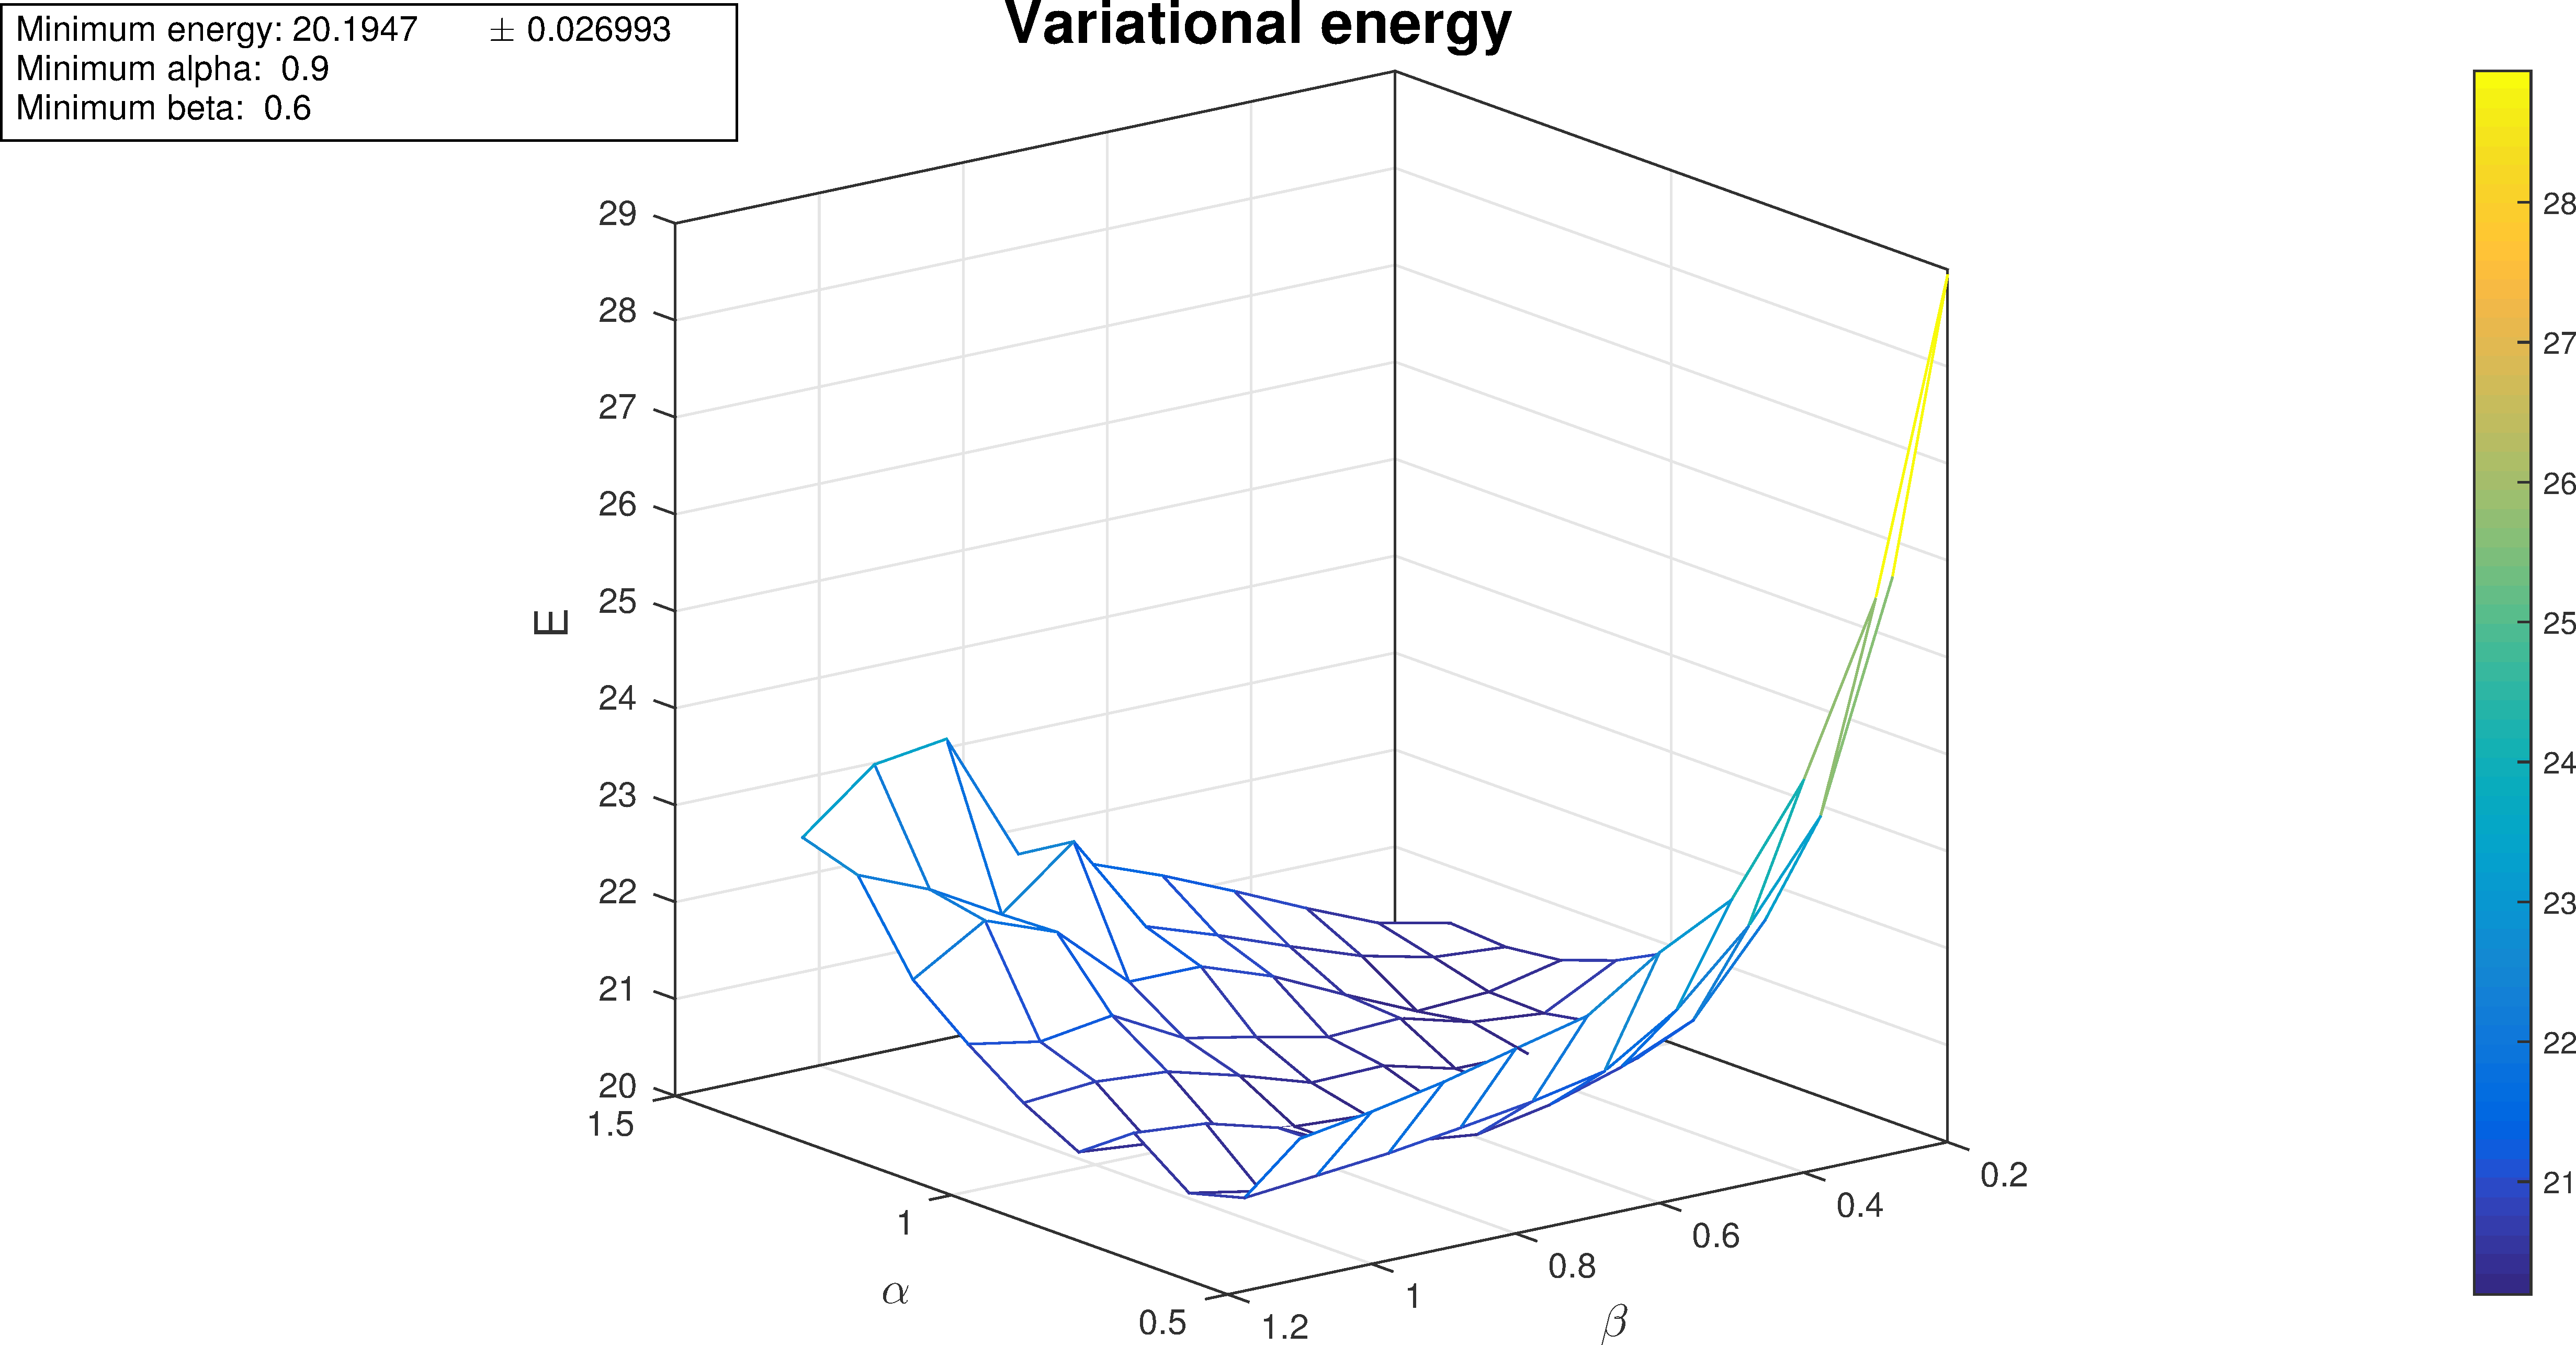
\includegraphics[width=\textwidth]{6e-100-rep}
	\end{figure}
	
	\note{		
		The variational energy versus the variational parameters $\alpha$ and $\beta$. The settings used are: importance sampling with $\Delta t = 0.1$, Jastrow factor, parallelization (8 threads), $10$ variations of $\alpha$ and $\beta$ with step $0.1$, $\SI{2e5}{}$ Monte Carlo steps. $\omega=1.00$.
		
		Our result is in very good accordance with the one calculated by DMC, that is $\SI{20.1597 \pm 0.0002}{\atomicunit}$.
	}

\end{frame}

\begin{versionLONG}

\section{Analytical derivatives}

\begin{frame}{Analytical derivatives}

	\uncover<+->{\emph{Idea:} speed up the calculation of the acceptance ratio by performing analytical derivatives.}
	
	\uncover<+->{Remember that}
	
	\uncover<+->{
		\begin{equation}
			\psi_T = |S^{\uparrow}||S^{\downarrow}|J
		\end{equation}
	}
	
	and
	
	\uncover<+->{
		\begin{equation}
			\vec{F}_i = 2\frac{1}{\psi_T}\nabla_i\psi_T,
			\qquad
			E_L = \frac{1}{2}\sum_{i}\frac{1}{\psi_T}\nabla^2_i\psi_T + \sum_i V_i.
		\end{equation}
	}
	
\end{frame}

\begin{frame}{Analytical derivatives}

	\uncover<+->{Doing the calculations}
	
	\uncover<+->{
		\begin{equation}
			\frac{1}{\psi_T}\nabla_i\psi_T
			= \frac{\nabla_{i}|S^{\alpha}|}{|S^{\alpha}|} + \frac{\nabla_{i}J}{J}
		\end{equation}
	}
	
	\uncover<+->{and}
	
	\uncover<+->{
		\begin{equation}
			\frac{1}{\psi_T}\nabla^2_i\psi_T
			= \frac{\nabla_i^2 |S^{\alpha}|}{|S^{\alpha}|}+\frac{\nabla^2_i J}{J}+2 \frac{\nabla_i |S^{\alpha}|}{|S^{\alpha}|}\frac{\nabla_i J}{J},
		\end{equation}
	}
	
	\uncover<+->{where $\alpha$ is the spin relative to particle $i$.}

\end{frame}

\begin{frame}{Analytical derivatives}

	\uncover<+->{Further simplifications give}
	
	\begin{align}
		\onslide<+->{\frac{\nabla_i J}{J} 
		&= \sum_{k \neq i=1}^N \frac{a_{ik}}{r_{ik}} \frac{\vec{r}_i-\vec{r}_k}{(1+\beta \, r_{ik})^2} \\}
		\onslide<+->{\frac{\nabla_i^2 J}{J} 
		&= \left|\frac{\nabla_i J}{J} \right|^2+ \sum_{k \neq i=1}^N a_{ik} \frac{(d-3)(\beta \, r_{ik}+1)+2}{r_{ik}(\beta \, r_{ik}+1)^3} \\}
		\onslide<+->{\frac{\nabla_i |S|}{|S|} 
		&= \sum_k \nabla_i \phi_k (\vec{r}_i^{\text{new}})(S_{ki}^{\text{new}})^{-1} \\}
		\onslide<+->{\frac{\nabla_i^2 |S|}{|S|} 
		&= \sum_k \nabla_i^2 \phi_k (\vec{r}_i^{\text{new}})(S_{ki}^{\text{new}})^{-1} \\}
		\notag
	\end{align}
	\vskip-1.5em

\end{frame}

\begin{frame}{Execution times -- 2 electrons}

	\begin{figure}
		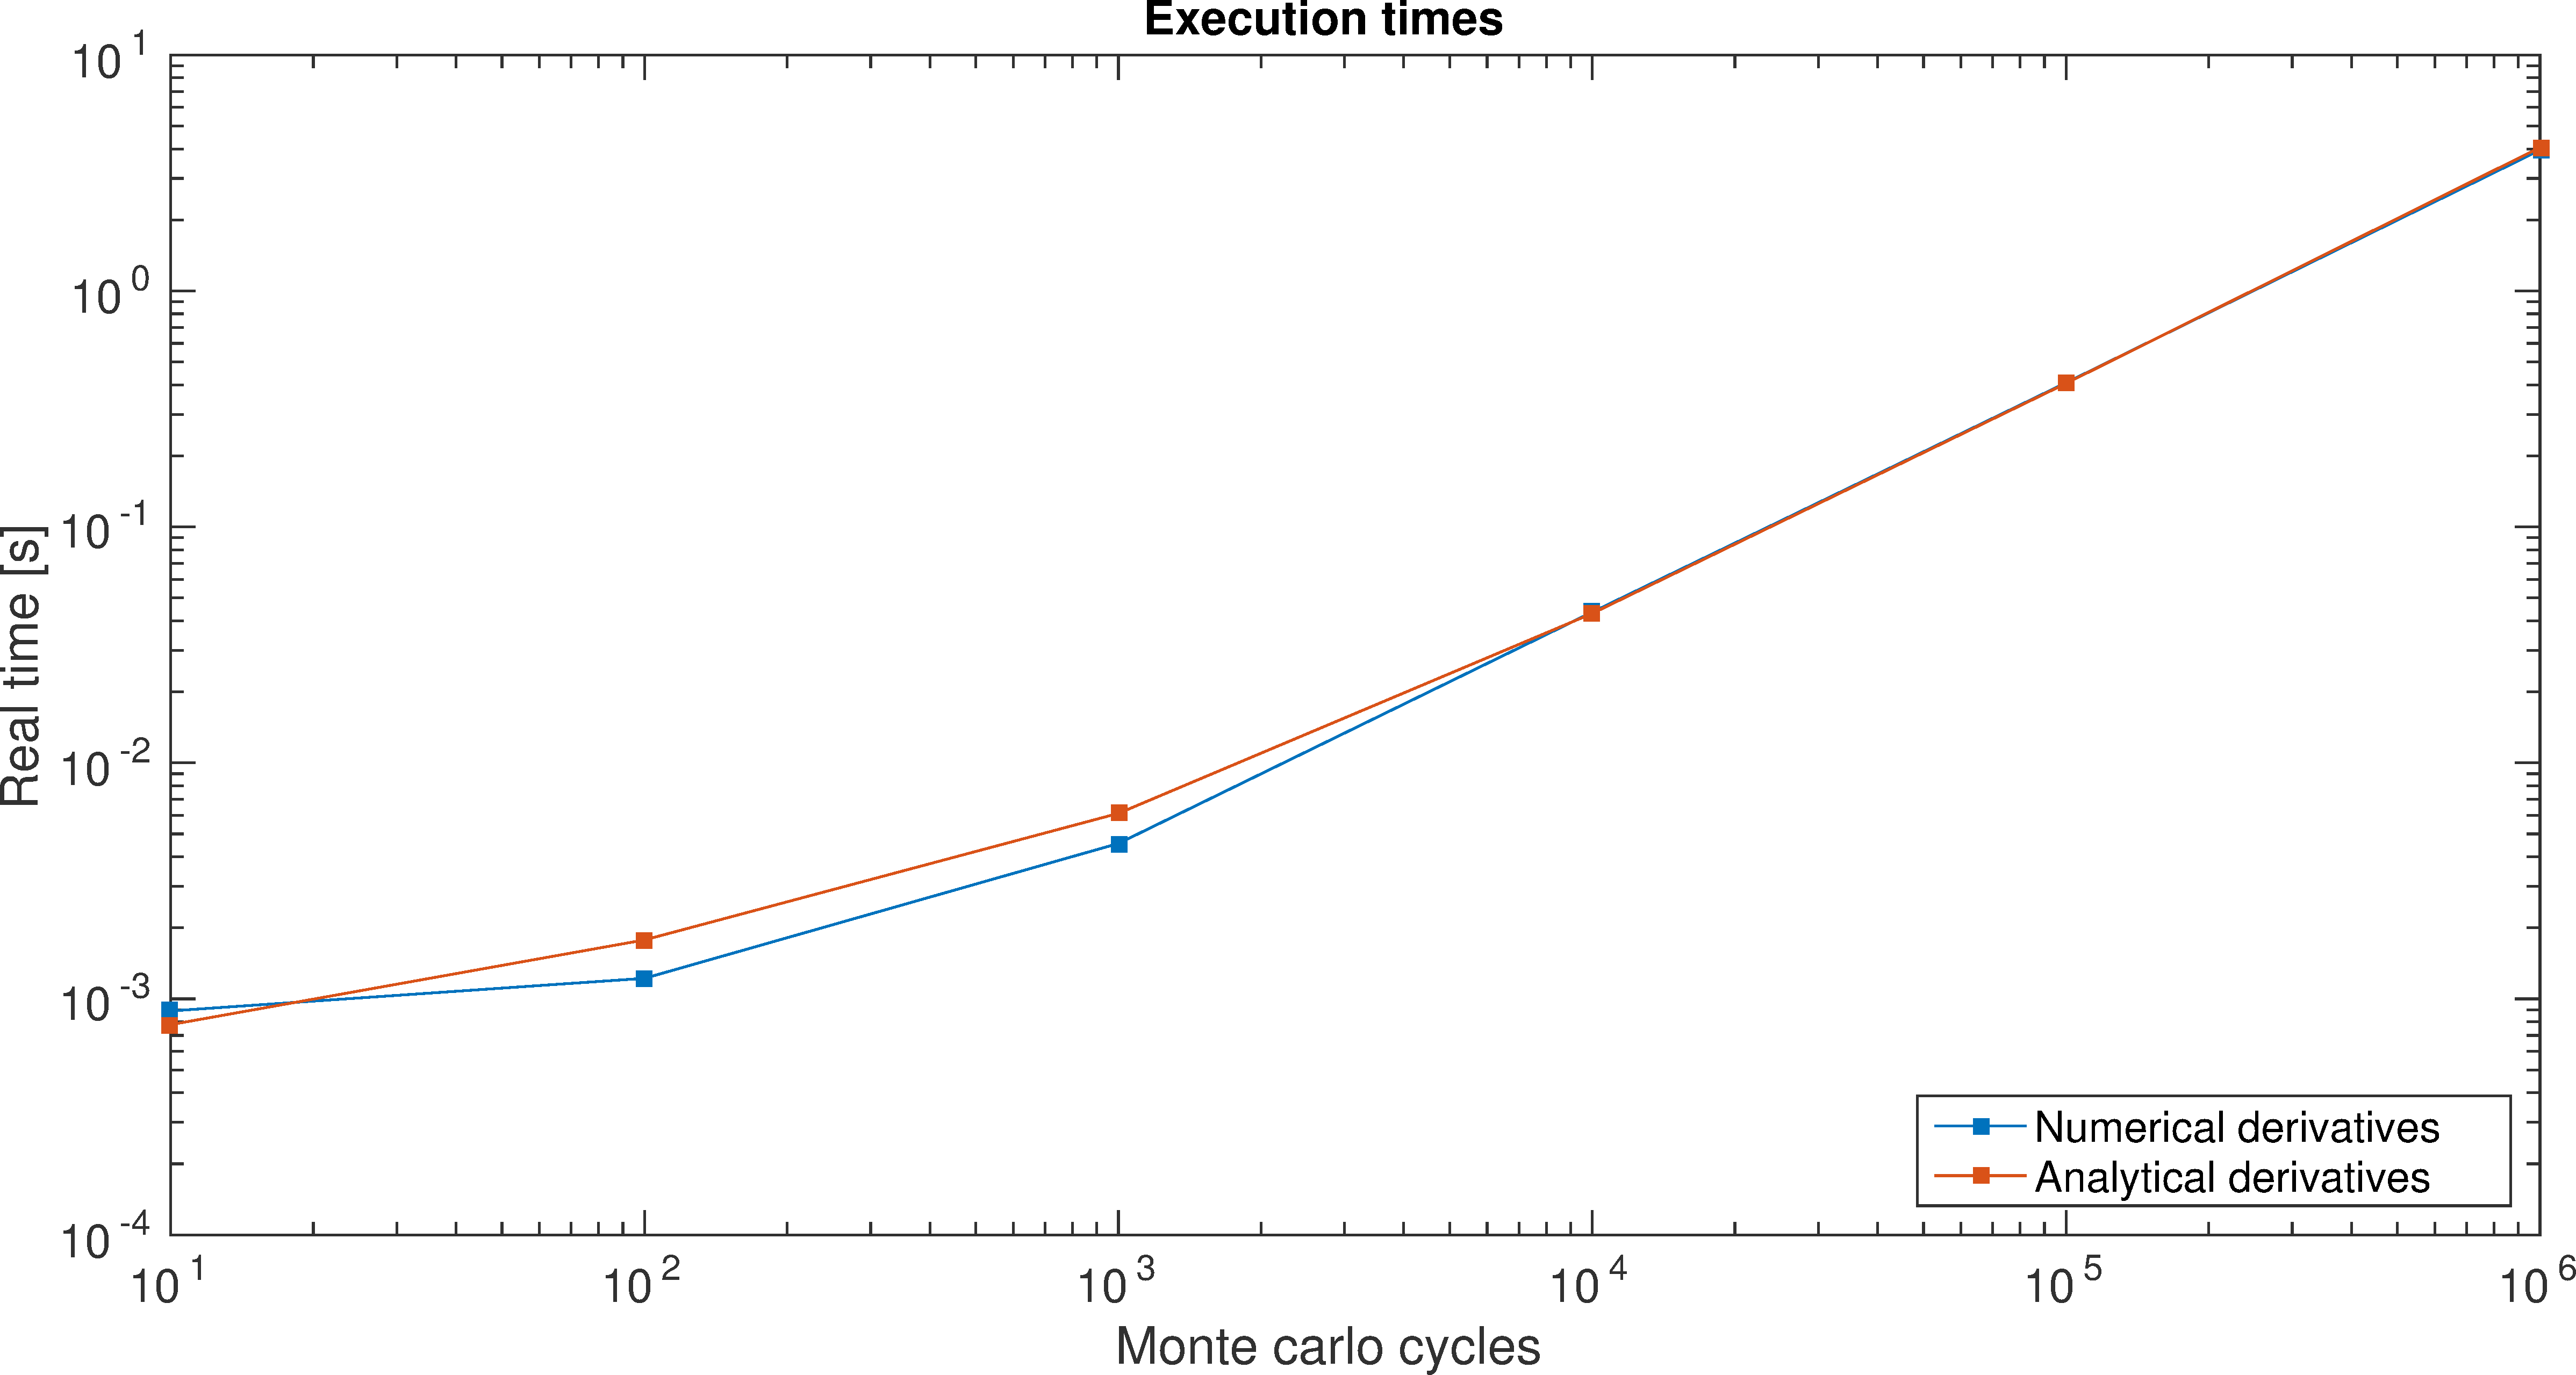
\includegraphics[width=\textwidth]{times_2e}
	\end{figure}
	
	\note{
		Execution times for 2-electrons and a single pair of variational parameters $(\alpha,\beta)$. The GNU/Linux system tool \texttt{time} was used to take the measurements.
	}

\end{frame}

\begin{frame}{Execution times -- 6 electrons}

	\begin{figure}
		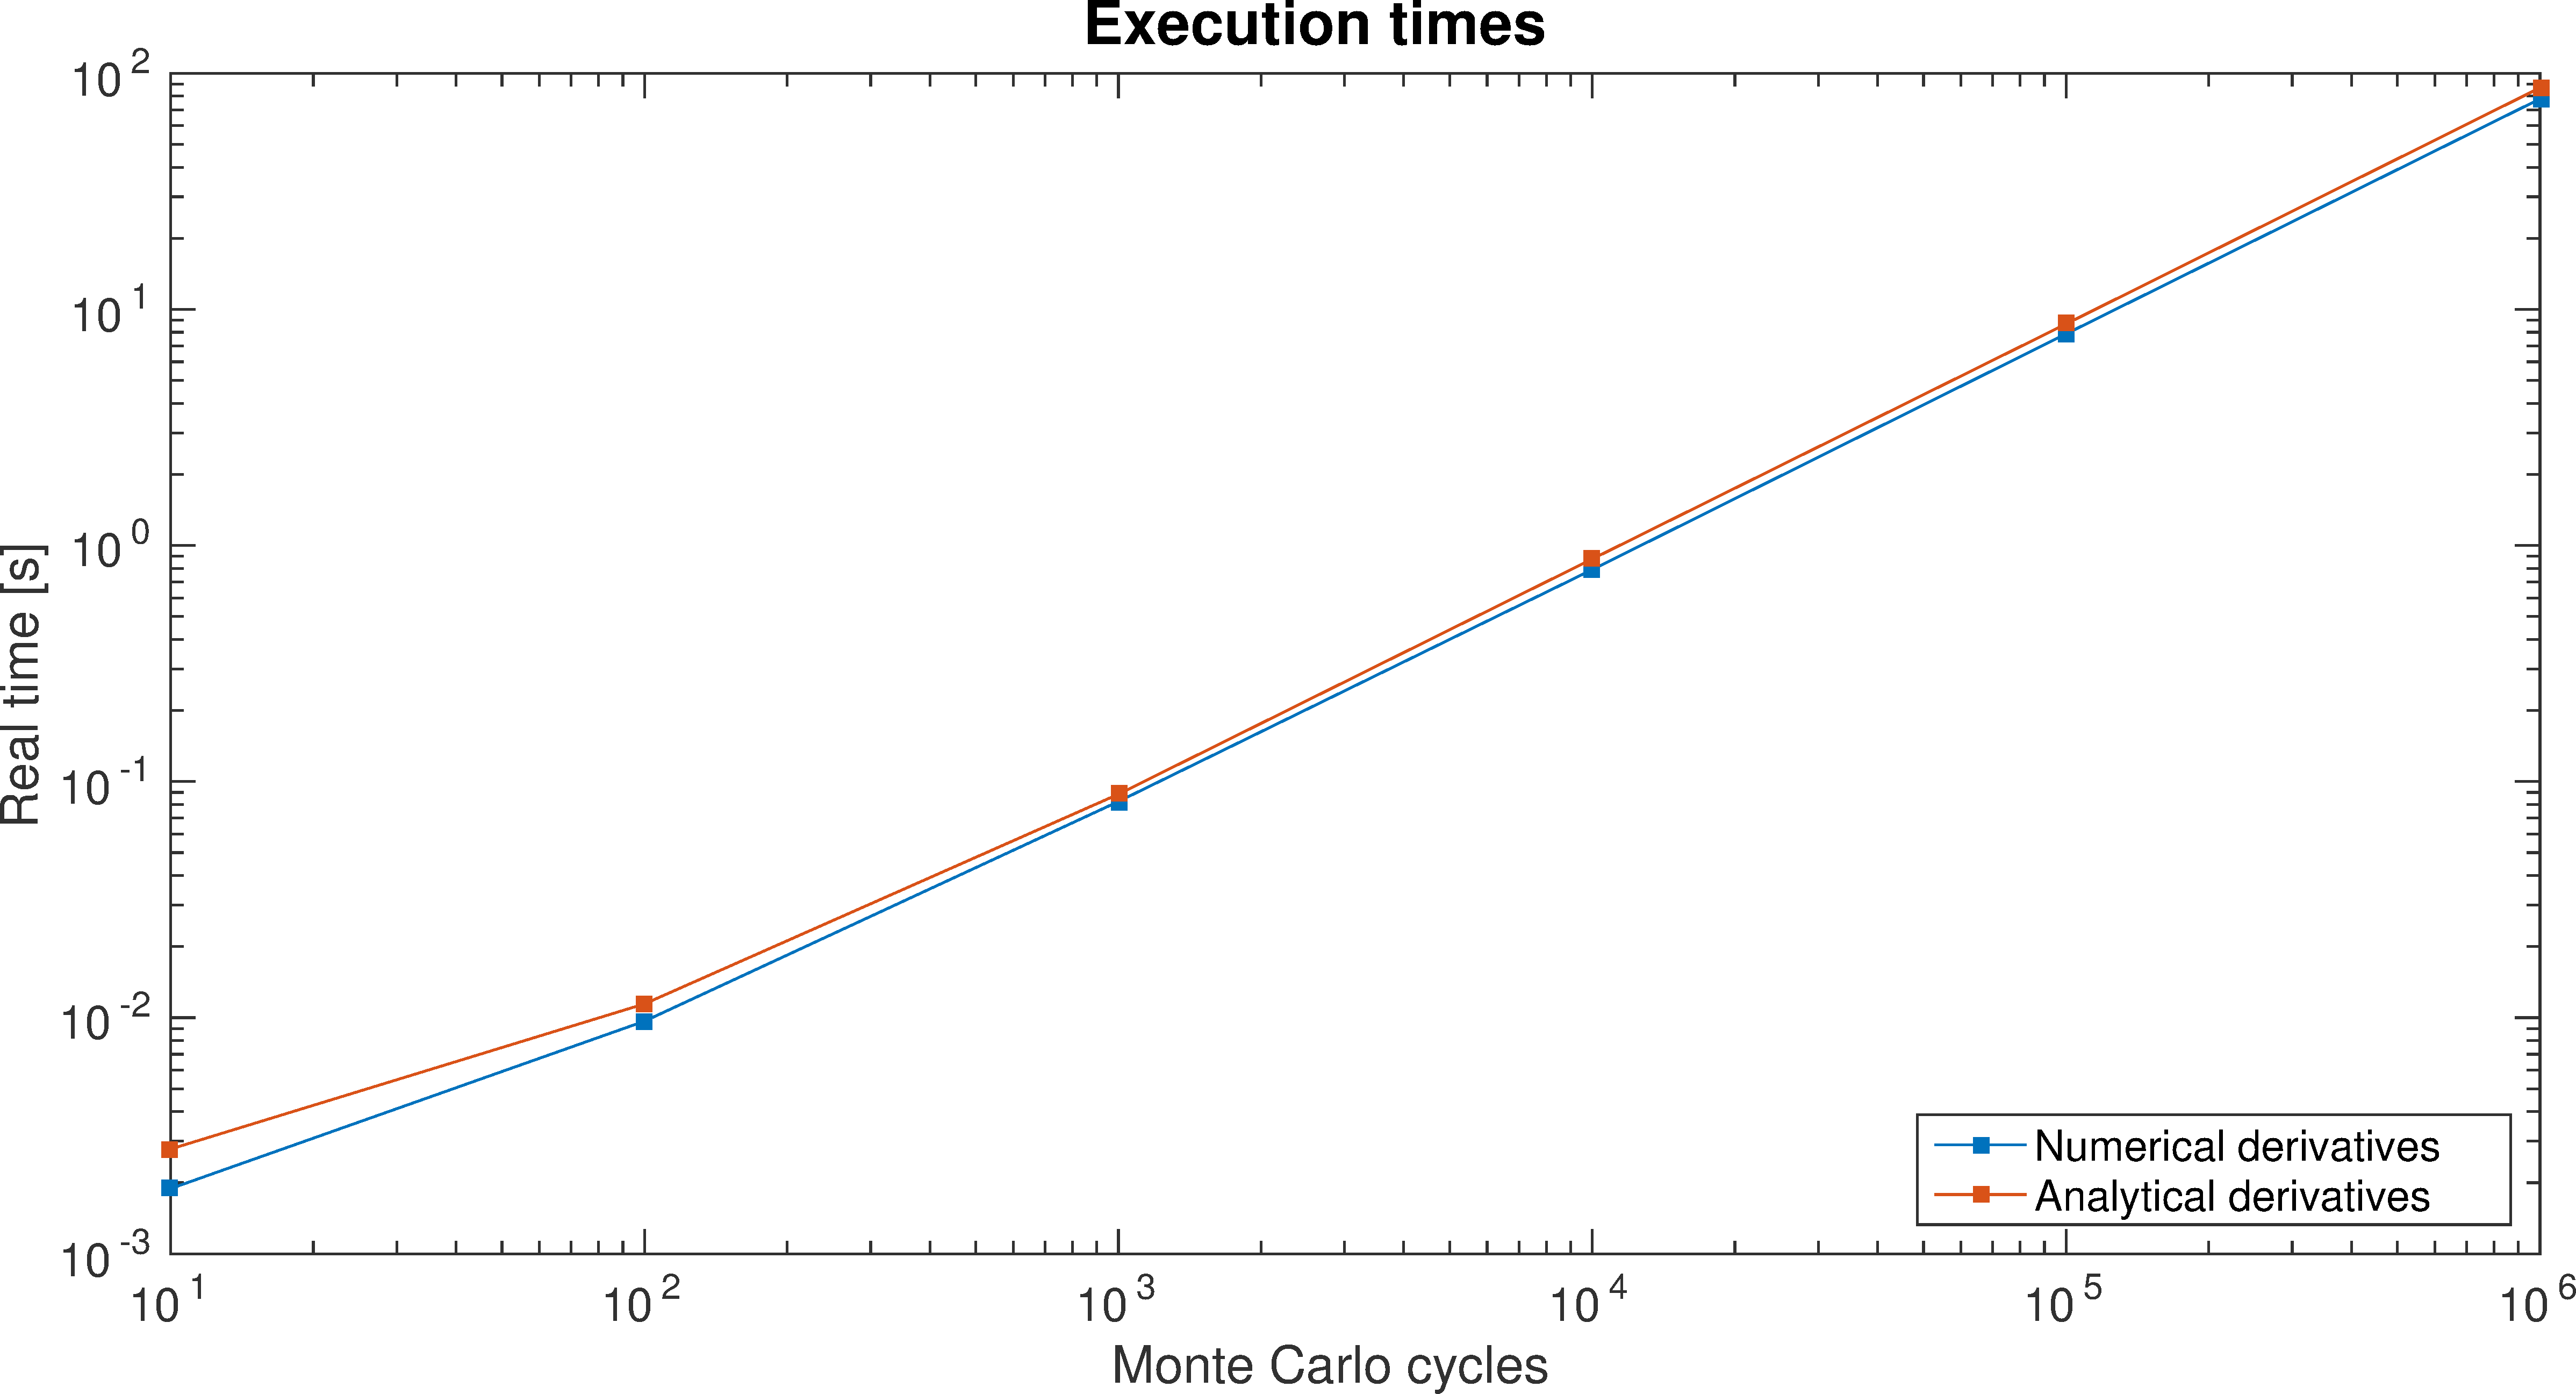
\includegraphics[width=\textwidth]{times_6e}
	\end{figure}
	
	\note{
		Execution times for 6-electrons and a single pair of variational parameters $(\alpha,\beta)$. The GNU/Linux system tool \texttt{time} was used to take the measurements.		
	}

\end{frame}

\begin{frame}{Comments}

	\begin{itemize}[<+->]
		\item We don't really have great improvements.
		\item We are performing a \emph{numerical inversion of a matrix} ($\sim\mathcal{O}(n^3)$).
		\item There is no optimization of the acceptance ratio.
		\item The determinant of a matrix has a computational complexity of $\sim\mathcal{O}(n^3)$, so we might not see improvements up to 12-20 particles.
	\end{itemize}

\end{frame}

\end{versionLONG}

\section{Conclusion}

\begin{frame}{Summary}

	\begin{itemize}[<+->]
		\item The VMC technique is an easy-to-implement tool that gives an upper bound to the ground state energy of a system.
		\item Although is used as a starting point for DMC calculations, if we choose our trial wave-function in a smart way this technique gives an upper bound that is surprisingly compatible with the actual ground-state energy.
		\item For $N$ interacting electrons in an attractive potential, a good approximation of the actual wave-function is
		\begin{equation*}
			\psi_T(\vec{r}_1,\ldots,\vec{r}_N) = |S^{\uparrow}||S^{\downarrow}|J
		\end{equation*}
		\item For a quantum dot, the calculations can be further simplified by analytical means.
		\item In general, such a simplification is not possible; what one does is to optimize the code and to parallelize it as much as possible via OpenMP/MPI and possibly GPU parallelization.
		\item \alert{Thanks for your attention!}
	\end{itemize}

\end{frame}

\plain{Questions?}

\end{document}
